% **************************************************
% Document Class Definition
% **************************************************
\documentclass[%
    paper=A4,               % paper size --> A4 is default in Germany
    twoside=true,           % onesite or twoside printing
    openright,              % doublepage cleaning ends up right side
    parskip=full,           % spacing value / method for paragraphs
    chapterprefix=true,     % prefix for chapter marks
    11pt,                   % font size
    headings=normal,        % size of headings
    bibliography=totoc,     % include bib in toc
    listof=totoc,           % include listof entries in toc
    titlepage=on,           % own page for each title page
    captions=tableabove,    % display table captions above the float env
    chapterprefix=false,    % do not display a prefix for chapters
    appendixprefix=false,   % but display a prefix for appendix chapter
    draft=false,            % value for draft version
]{scrreprt}%


% **************************************************
% Setup YOUR thesis document in this file !
% **************************************************
% !TEX root = main.tex


% **************************************************
% Files' Character Encoding
% **************************************************
\PassOptionsToPackage{utf8}{inputenc}
\usepackage{inputenc}


% **************************************************
% Information and Commands for Reuse
% **************************************************
\newcommand{\thesisTitle}{SerialExperimentsOlga}
\newcommand{\thesisName}{Olga Yakobson}
\newcommand{\thesisSubject}{Bachelor’s Thesis}
\newcommand{\thesisDate}{February 4, 2022}
\newcommand{\thesisVersion}{My First Draft}

\newcommand{\thesisFirstReviewer}{Prof.~Dr.~Eyke Hüllermeier}
\newcommand{\thesisFirstReviewerUniversity}{\protect{LMU Munich}}
\newcommand{\thesisFirstReviewerDepartment}{Institute of Informatics}

\newcommand{\thesisSecondReviewer}{John Doe}
\newcommand{\thesisSecondReviewerUniversity}{\protect{LMU Munich}}
\newcommand{\thesisSecondReviewerDepartment}{Institute of Informatics}

\newcommand{\thesisFirstSupervisor}{Jane Doe}
\newcommand{\thesisSecondSupervisor}{John Smith}

\newcommand{\thesisUniversity}{LMU Munich}
\newcommand{\thesisUniversityDepartment}{Department of Mathematics, Informatics and Statistics}
\newcommand{\thesisUniversityInstitute}{Institute of Informatics}
\newcommand{\thesisUniversityGroup}{Artificial Intelligence and Machine Learning (AIML)}
\newcommand{\thesisUniversityCity}{Munich}
\newcommand{\thesisUniversityStreetAddress}{Akademiestra\ss e 7}
\newcommand{\thesisUniversityPostalCode}{80799 Munich}


% **************************************************
% Debug LaTeX Information
% **************************************************
%\listfiles


% **************************************************
% Load and Configure Packages
% **************************************************
\usepackage[english]{babel} % babel system, adjust the language of the content
\PassOptionsToPackage{% setup clean thesis style
    figuresep=colon,%
    hangfigurecaption=false,%
    hangsection=true,%
    hangsubsection=true,%
    sansserif=false,%
    configurelistings=true,%
    colorize=full,%
    colortheme=lmuaiml,%
    configurebiblatex=true,%
    bibsys=biber,%
    bibfile=bib-refs,%
    bibstyle=alphabetic,%
    bibsorting=nty,%
}{cleanthesis}
\usepackage{cleanthesis}
\usepackage[nottoc]{tocbibind}
\usepackage{mathtools}
\usepackage{amssymb}
\usepackage{amsthm}
\usepackage{thmtools}
\usepackage{bm}
\usepackage{bbm}
\usepackage{dsfont}
\usepackage{centernot}
\usepackage{breqn}
\usepackage{nicefrac}
\usepackage{wasysym}
\usepackage{arydshln}
\usepackage{algorithm}
\usepackage{algpseudocode}
\usepackage{algorithmicx}
\usepackage{siunitx}
\usepackage{tabu}
\usepackage{csvsimple}
\usepackage{multicol}
\usepackage{multirow}
\usepackage{booktabs}
\usepackage{dsfont}



\algrenewcommand\algorithmicrequire{\textbf{Input:}}
\algrenewcommand\algorithmicensure{\textbf{Output:}}
\newcommand\numberthis{\addtocounter{equation}{1}\tag{\theequation}}
\newcommand*{\dblbrace}[2][]{#1{#2}\ifthenelse{\equal{#1}{}}{\mskip-6mu}{\mskip-8mu}#1{#2}}
\newcommand*{\ldblbrace}[1][]{\dblbrace[#1]{\{}}
\newcommand*{\rdblbrace}[1][]{\dblbrace[#1]{\}}}
\newcommand*\dif{\mathop{}\!\mathrm{d}}

\hypersetup{% setup the hyperref-package options
    pdftitle={\thesisTitle},    %   - title (PDF meta)
    pdfsubject={\thesisSubject},%   - subject (PDF meta)
    pdfauthor={\thesisName},    %   - author (PDF meta)
    plainpages=false,           %   -
    colorlinks=false,           %   - colorize links?
    pdfborder={0 0 0},          %   -
    breaklinks=true,            %   - allow line break inside links
    bookmarksnumbered=true,     %
    bookmarksopen=true          %
}

% **************************************************
% Other Packages
% **************************************************
\usepackage{amsfonts}
\usepackage{scrhack}
\usepackage{lipsum}
\usepackage{tikz}% do not disable this package
\usetikzlibrary{backgrounds,calc}
\usepackage{cleveref}
\usepackage{acro}
\usepackage{amsthm}
\usepackage{array} % overleaf
\usepackage{multirow} % overleaf
\usepackage{pgfplots}
\usepackage{xcolor}
\acsetup{
    %first-long-format=\slshape,
    barriers/use=true
}


% Colors:
\definecolor{t_blue}{HTML}{355fb3}
\definecolor{t_red}{HTML}{b33535}
\definecolor{t_green}{HTML}{3bb335}
\definecolor{t_yellow}{HTML}{b39735}
\definecolor{t_darkblue}{HTML}{1e3666}
\definecolor{t_darkgreen}{HTML}{22661e}
\definecolor{t_darkred}{HTML}{661e1e}
\definecolor{t_darkyellow}{HTML}{66571e}
\definecolor{t_lightblue}{HTML}{8ea7d7}
\definecolor{t_lightred}{HTML}{dc8989}
\definecolor{t_lightgreen}{HTML}{8ddc89}
% Colors specifically for plots 
\definecolor{p_red}{HTML}{b33535}
\definecolor{p_green}{HTML}{355fb3}
\definecolor{p_blue}{HTML}{3bb335}
\definecolor{p_yellow}{HTML}{b39735}
\definecolor{p_violet}{HTML}{9235B3}
% **************************************************
% Custom Macros
% **************************************************
\newcommand{\dac}[3]{\DeclareAcronym{#1}{short = #2, long = #3}}

% Custom commands:
\renewcommand{\labelitemi}{\raisebox{.4\height}{\textcolor{t_darkblue}{\scriptsize$\blacktriangleright$}}}
\newcommand{\tikzmark}[1]{\tikz[overlay,remember picture] \node (#1) {};} % chktex 1
\newcommand*\circled[2][1pt]{\tikz[baseline=(char.base)]{ % chktex 36
        \node[shape=circle,draw,inner sep=#1] (char) {#2};}}
\newcommand*{\badgeboxinline}[2][black]{\fcolorbox{#1}{white}{\textsf{%
            \small\,% chktex 21
            \ifthenelse{\equal{\detokenize{#1}}{\detokenize{t_yellow}}}{\textcolor{t_darkyellow}{#2}}{%
                \ifthenelse{\equal{\detokenize{#1}}{\detokenize{t_green}}}{\textcolor{t_darkgreen}{#2}}{\textcolor{#1}{#2}}%
            }\,}}} % chktex 21
\newcommand*{\badgebox}[2][black]{\hspace*{\fill}\badgeboxinline[#1]{#2}}
\newcommand{\cmark}{\ding{51}}
\newcommand{\xmark}{\ding{55}}
\providecommand\rightarrowRHD{\mathrel{\relbar\mathrel{\mkern-8mu\RHD}}}
\newcommand*\linksym{\includegraphics[height=1.4ex]{gfx/link.pdf}\mkern1mu}
\newcommand*{\colorlabel}[2]{\textsf{\textbf{\small\textcolor{#1}{#2}}}}
\newcommand*{\condbold}[3][]{\ifthenelse{\equal{#2}{1}#1}{\mathbf{#3}}{#3}}
\def\evalprec{2}
\newcommand*{\evalres}[4][]{%
    \ifthenelse{\equal{#3}{m}}{\acs*{oom}}{%
        \ifthenelse{\equal{#3}{t}}{\acs*{oot}}{$\condbold[#1]{#2}{\num[round-mode=places,round-precision=\evalprec]{#3}} \pm \num[round-mode=places,round-precision=\evalprec]{#4}$}}%
}

\newcommand{\sourceinline}[2][source]{{\scriptsize\textsc{#1:~\cite{#2}}}}
\newcommand{\source}[2][source]{\hspace*{\fill}\sourceinline[#1]{#2}}
\newcommand{\cfullref}[2][, ]{\cref{#2}#1\cpageref{#2}}

\newcounter{daggerfootnote}
\newcommand*{\daggerfootnote}[1]{%
    \setcounter{daggerfootnote}{\value{footnote}}%
    \renewcommand*{\thefootnote}{\fnsymbol{footnote}}%
    \footnote[2]{#1}%
    \setcounter{footnote}{\value{daggerfootnote}}%
    \renewcommand*{\thefootnote}{\arabic{footnote}}}

\preto\tabular{\setcounter{rownumbercount}{0}}
\newcounter{rownumbercount}
\newcommand\rownumber{\stepcounter{rownumbercount}\arabic{rownumbercount}}

\DeclareMathOperator{\Tr}{Tr}
\DeclareMathOperator{\mean}{mean}
\DeclareMathOperator{\wmean}{wmean}
\DeclareMathOperator{\wmaj}{wmaj}
\DeclareMathOperator{\sgn}{sgn}
\DeclareMathOperator{\set}{set}
\DeclareMathSymbol{\shortminus}{\mathbin}{AMSa}{"39} % chktex 18

\theoremstyle{plain}
\newtheorem{thm}{Theorem}[chapter]
\newtheorem{prop}[thm]{Proposition}
\crefname{prop}{proposition}{propositions}
\Crefname{prop}{Proposition}{Propositions}
\newtheorem{lem}[thm]{Lemma}
\newtheorem{fact}[thm]{Fact}
\newtheorem{cor}[thm]{Corollary}

\theoremstyle{definition}
\newtheorem{defn}[thm]{Definition}








% Acronyms 

% General learners:
\dac{nn}{NN}{neural network}
\dac{lm}{LRM}{logistic regression model}
\dac{svm}{SVM}{support vector machine}
\dac{mlp}{MLP}{multilayer perceptron}
\dac{cnn}{CNN}{convolutional neural network}


% Networks 
\dac{gcr}{GC/GR}{graph classification and regression}
\dac{gc}{GC}{graph classification}
\dac{gr}{GR}{graph regression}
\dac{gk}{GK}{graph kernel}
\dac{gnn}{GNN}{graph neural network}
\dac{gcnn}{GCNN}{graph convolutional neural network}
\dac{gcn}{GCN}{graph convolutional network}
\dac{gin}{GIN}{graph isomorphism network}
\dac{nc}{NC}{node classification}
\dac{nr}{NR}{node regression}

% Regularization 
\dac{do}{DO}{DropOut}
\dac{de}{DE}{DropEdge}
\dac{ns}{NS}{NodeSampling}
\dac{gdc}{GDC}{GraphDropConnect}

% Theory:
\dac{ml}{ML}{machine learning}
\dac{xai}{XAI}{explainable artificial intelligence}
\dac{gi}{GI}{graph isomorphism}
\dac{wl}{WL}{Weisfeiler-Lehman}
\dac{ft}{FT}{Fourier transform}
\dac{bfs}{BFS}{breadth-first-search}
\dac{lcm}{LCM}{lowest common multiple}

% Experimental 
\dac{ogb}{OGB}{Open Graph Benchmark}
\dac{mad}{MAD}{Mean Average Distance}
\dac{madg}{MADGap}{MADGap}
\dac{gs}{GS}{grid search}
\bibliography{bib-refs.bib}

% **************************************************
% Document CONTENT
% **************************************************
\begin{document}

% --------------------------
% rename document parts
% --------------------------
%\renewcaptionname{ngerman}{\figurename}{Abb.}
%\renewcaptionname{ngerman}{\tablename}{Tab.}
\renewcaptionname{english}{\figurename}{Fig.}
\renewcaptionname{english}{\tablename}{Tab.}

% --------------------------
% Front matter
% --------------------------
\pagenumbering{roman}			% roman page numbing (invisible for empty page style)
\pagestyle{empty}				% no header or footers
% !TEX root = ../main.tex
%
% ------------------------------------  --> cover title page
\begin{titlepage}
	\pdfbookmark[0]{Cover}{Cover}
	\flushright
	\hfill
	\vfill
	{\LARGE\thesisTitle \par}
	\rule[5pt]{\textwidth}{.4pt} \par
	{\Large\thesisName}
	\vfill
	\textit{\large\thesisDate} %\\
	% Version: \thesisVersion
\end{titlepage}


% ------------------------------------  --> main title page
\begin{titlepage}
	\pdfbookmark[0]{Titlepage}{Titlepage}
	\tgherosfont


	\begin{figure}
		\begin{minipage}[t]{8.5cm}
			\includegraphics[height=1.8cm,width=4.25cm]{gfx/lmulogo.pdf}\\
			\textsf{\small{Department of Mathematics,  \\ Informatics and Statistics \\
					\thesisUniversityInstitute
					%		\textsf{\small{
					%		\hspace*{1.3cm}Warburger Straße 100 \\
					%		\hspace*{1.3cm}33098 Paderborn
				}}
		\end{minipage}
		\hfill
		\begin{minipage}[t]{4.7cm}
			\includegraphics[height=1.8cm,width=4.7cm]{gfx/aiml-logo-solid-black.pdf}\\
			\textsf{%Institute of Computer Science\\
				\hspace*{0.1cm}\small{Artificial Intelligence and \\ \hspace*{0.1cm}Machine Learning}
			}
		\end{minipage}
	\end{figure}

	\centering
	%\textsf{\thesisUniversityDepartment} \\
	%\textsf{\thesisUniversityInstitute} \\
	%\textsf{\thesisUniversityGroup} \\

	\vfill
	{\large \thesisSubject} \\[5mm]
	{\LARGE \color{ctcolortitle}\textbf{\thesisTitle} \\[10mm]}
	{\Large \thesisName} \\

	\vfill
	\begin{minipage}[t]{.27\textwidth}
		\raggedleft
		\textit{Reviewer}
	\end{minipage}
	\hspace*{15pt}
	\begin{minipage}[t]{.65\textwidth}
		{\Large \thesisFirstReviewer} \\
		{\small \thesisFirstReviewerDepartment} \\[-1mm]
		{\small \thesisFirstReviewerUniversity}
	\end{minipage} \\[5mm]

	\thesisDate\\

	\begin{tikzpicture}[remember picture,overlay]
		\begin{pgfonlayer}{background}
			\node[anchor=south east,outer sep=0pt,inner sep=0pt] at ($(current page.south east) +(-0in,0in)$) {\includegraphics[trim=0 55 100 00,clip,width=0.2\paperheight,height=0.25\paperheight]{gfx/siegel.pdf}};
		\end{pgfonlayer}
	\end{tikzpicture}

\end{titlepage}


% ------------------------------------  --> lower title back for single page layout




\hfill
\vfill
{
	\small
	\textbf{\thesisName} \\
	\textit{\thesisTitle} \\
	\thesisSubject, \thesisDate \\
	Reviewer: \thesisFirstReviewer \\
	Supervisor: \thesisFirstSupervisor\\[1.5em]
	\textbf{\thesisUniversity} \\
	\thesisUniversityDepartment \\
	\thesisUniversityInstitute \\
	\textit{\thesisUniversityGroup} \\
	\thesisUniversityStreetAddress \\
	\thesisUniversityPostalCode\
}
		% INCLUDE: all titlepages
\cleardoublepage

\pagestyle{plain}				% display just page numbers
% !TEX root = ../main.tex
%
\pdfbookmark[0]{Abstract}{Abstract}
\chapter*{Abstract}
\label{sec:abstract}
\vspace*{-10mm}

This thesis considers the effectiveness of regularization in the research field of graph classification and regression tasks to solve the problem of overfitting and over-smoothing. %, which are very common problems occurring in \acfp{gnn}.
The performance of four types of regularization techniques is evaluated and shown to be ineffective on two types of \ac{gnn} network architectures \ac{gcn} and \ac{gin} across five different molecular \ac{ogb} datasets. The similarity between \ac{gdc} and \ac{de} is highlighted.
We show that the evaluated \ac{gnn} architectures are unaffected by the problem of over-smoothing on graph-level tasks, and the overfitting aspect is shown to be unmitigated by regularization.

% \vspace*{20mm}

% {\usekomafont{chapter}Abstract (different language)}\label{sec:abstract-diff} \\

		% INCLUDE: the abstracts (english and german)
\cleardoublepage
%
% !TEX root = ../main.tex
%
% \pdfbookmark[0]{Acknowledgement}{Acknowledgement}
% \chapter*{Acknowledgement}
% \label{sec:acknowledgement}
% \vspace*{-10mm}

 % INCLUDE: acknowledgement
\cleardoublepage
%
\currentpdfbookmark{\contentsname}{toc}
\setcounter{tocdepth}{2}		% define depth of toc
\tableofcontents				% display table of contents
\cleardoublepage

% --------------------------
% Body matter
% --------------------------
\acbarrier
\pagenumbering{arabic}			% arabic page numbering
\setcounter{page}{1}			% set page counter
\pagestyle{scrheadings} 	% fancy header and footer

% !TEX root = ../main.tex
% chktex-file 46
\chapter{Introduction}%
\label{sec:intro}

\pagenumbering{arabic}			% arabic page numbering
\setcounter{page}{1}			% set page counter

The field of \acs{ml} on graph-structured data has recently become an active topic of research.
One reason for this is the wide range of domains and problems that are expressible using graphs.
Regularization techniques are commonly employed in node-level prediction tasks across diverse networks to mitigate overfitting and over-smoothing, a condition where the performance and predictive power of a \ac{nn} do not improve or even get worse when more layers are added. % TODO: cite 
These methods perturb the values and introduce randomness, leading to improved results.
In graph-level tasks, however, the final output is a readout of aggregated nodes, hypothetically minimizing the impact of over-smoothing as the emphasis shifts from distinguishing individual nodes to capturing collective behavior.


\section{Motivation}%
\label{sec:intro:motivation}
% Mention GDC (including citation!)

The exploration of controlled randomness in graph-level prediction tasks may initially appear unconventional since the focus shifts from individual nodes to capturing the collective behavior of the graph.
The usual thinking about graph-level predictions might question if we need controlled randomness.
Since the last step in graph-level prediction models is a readout operation, which combines the whole graph or a subgraph structure,
the attention shifts from distinguishing individual nodes to the representation of the entire graph, making over-smoothing potentially less problematic.
Despite this counterintuitive aspect, our study aimed to empirically validate the effectiveness of regularization techniques in graph-level prediction tasks.
Our curiosity was motivated by a desire to challenge existing assumptions and gain a nuanced understanding of the relationship between regularization methods and graph-level predictions.
In this pursuit, we aim to extend the boundaries of understanding regarding the impact of regularization on aggregated outcomes.
One noteworthy technique that caught our attention was \acf{gdc}, which introduces stochasticity through adaptive connection sampling \cite{Hasanzadeh2020}.
By drawing different random masks for each channel and edge independently, \ac{gdc} promises to provide nuanced improvements, surpassing the effectiveness of traditional methods or even their combinations.
Also, we want to better understand the role of controlled randomness in the context of overfitting and over-smoothing by evaluating four regularization techniques.

\section{Research Questions}%
\label{sec:intro:questions}
In this thesis, we will answer the following research questions to assess the relevance of regularization for graph-level prediction tasks:
\begin{enumerate}
    \item Is regularization, specifically \ac{gdc}, effective in solving the problem of overfitting and over-smoothing for graph-level prediction tasks?
    \item Is there a difference in performance between \ac{gcn} and \ac{gin} architectures regarding performance with regularization techniques?
    \item Are there similarities and differences between different regularization techniques in terms of performance?
\end{enumerate}
\section{Structure}%
\label{sec:intro:structure}

\paragraph{\Cref{sec:related}: \nameref{sec:related}}
In order to answer our three research questions, we first take a closer look at three common prediction tasks in \acp{gnn}
and give a general overview of how \acp{gnn} organize and process graph-structured data.
We discuss the relation of the message-passing mechanism to the \ac{wl}-test and give a formal definition and description of two \acp{gnn} architectures, \ac{gcn} and \ac{gin}, before taking a closer look at typical issues occurring in \acp{gnn}.
Finally, we present four regularization techniques, which mitigate two commonly occurring problems and \acf{mad}, a measure for smoothness between nodes~\cite{Chen2020}.
% Problem Description + Implementation = implement 
\paragraph{\Cref{sec:implement}: \nameref{sec:implement}}
This section overviews the implementation of graph convolutions using TensorFlow's \texttt{gather} and \texttt{scatter} operations.
We then explain how we implement four regularization techniques by masking values during different convolution steps.
We provide an intuitive approach for looking at \ac{gdc}.
Lastly, we discuss the benefits of using \ac{ogb} datasets.
% eval contains discussion 
\paragraph{\Cref{sec:eval}: \nameref{sec:eval}}
We start with an overview of used datasets and metrics before proceeding to the experimental setup.
We then describe our parameter grid and explain how we choose the best set of hyperparameters.
Finally, we present the experimental results and provide insights into how different numbers of layers and probability affect the performances of \ac{gnn} and \ac{gin} and draw a conclusion from our findings.
\paragraph{\Cref{sec:conclusion}: \nameref{sec:conclusion}}
Finally, the results of this thesis are summarized, and a brief outline of promising directions for future research is given.
   % INCLUDE my_intro
% !TEX root = ../main.tex
%
\chapter{Related Work}
\label{sec:related}

% feedback-appl
Before describing the problem, and later on the experimental setup, we first
\begin{enumerate}
    \item Introduce three common prediction tasks in \acp{gnn}.
    \item Give a general overview of how \acp{gnn} organize and process graph structured data.
    \item We further discuss the relation of messasge passing mechanism to the WL-test, an algorithm for
          inspecting whether two graphs are isomorph.
    \item Give a formal definition and description of two \ac{gnn}
          architectures which will be used in our experiments.
    \item Discuss typical issues which occur in \acp{gnn} and methods for adressing those issues.
\end{enumerate}


\section{Prediction Tasks and Typical Problems}
\label{sec:related:pred}

% Types of prediction tasks (free-by-me) READY
Graphs naturally appear in numerous application domains, ranging from social analysis, bioinformatics to computer vision.
A Graph $G = (V,E)$, where $V = \{v_{1},...,v_{n}\}$ is a set of $N =|V|$ nodes and $E \subseteq V\times V$ a set of edges betwen those nodes. The unique capability of graphs enables capturing the structural relations among data, and thus allows to harvest more insights compared to analyzing data in isolation~\cite{Zhang19}. Graphs therefore can be seen as a general language for describing entities and relationships between those entities.
\Acfp{gnn} then organize graph structured data to tackle various prediction and classification
tasks. Typically, one is interested in one of the following three tasks:
\begin{enumerate}[label=\textbf{\arabic*.}]
    \item \textbf{Link prediction:}
          Predict whether there are missing links between two nodes
          e.g., knowledge graph completion.

    \item \textbf{Vertex classification \& regression:}
          Predict a property of a node e.g., categorize online users/items.

    \item \textbf{Graph classification \& regression:}
          Here, we are interested in classifying or predicting a continuous value for
          the entire graph, e.g., predicting a property of a molecule.
\end{enumerate}

In this work the main focus will be on \ac{nc}, \ac{gc} and \ac{gr} for small- as well as medium-sized graphs.

% Message passing formally
\section{Passing Messages in \Acsp*{gnn}}
\label{sec:related:message}

% Intro to GNNs, State-description (free-by-me) READY
Graphs, by nature, are unstructured. Vertices in graphs have no natural order and can
contain any type of information. In order for machine learning algorithms to be able
to make use of graph structured data, a mechanism is needed to organize them in a
suitable way~\cite{Zhou2020a,Hamilton2017a,Zhang19}.


% Message Passing in general (free-by-me) READY
Message passing is a mechanism, which embeds into every node information about it's neighbourhood ~\cite{Xu2019,Zhou2020a}. This can be done in several ways. One way of classifying a \ac{gnn} is by looking at the underlying message passing machanism. In this paper we will look at a network, where message passing is done via convolutions (\acf{gcn}). We will however ocasionally use the more general term message passing, as the separation is rather blurred and message passing describes a neighborhood aggregation scheme which is seen as a generalisation of other, more specific mechanisms.

Formally, message passing in a \ac{gnn} can be described as using two functions:
AGGREGATE and COMBINE. The expressive and representational power of a \ac{gnn} can
then be determined by looking at the concrete functions and their properties, used to implement
aggregation and combination. AGGREGATE mixes the hidden representation of every node's neighborhood in every iteration. COMBINE then combines the mixed representation togheter with the representation of the node. Each node uses the information from its neighbors to update its embeddings, thus a natural extension is to use the information to increase the receptive field by performing AGGREGATE and COMBINE multiple times.

\begin{align*}
    a_{v}^{k}   & = \mathrm{AGGREGATE}^{(k)}(\{h_{u}^{(k-1)}: u \in \mathcal{N}_{(v)}\}) \\
    h_{v}^{(k)} & = \mathrm{COMBINE}^{(k)}(h_{v}^{(k-1)}, a_{v}^{(k)})
\end{align*}

For graph-level predictions, an additional READOUT- operation is used:
\begin{align*}
    h_{G} =\mathrm{READOUT}(\{h_{v}^{(K)}\ \mid \ v \in G\})
\end{align*}

% Message passing framework and local graph structure (free-by-me) READY
One useful type of information, which the message passing framework should be able to
capture, is the local graph structure. This can be done by choosing functions with
appropriate properties. A more detailed explanation will follow in
\cref{sec:related:architectures}. In spatial \acp{gnn} we make the assumption of the
similarity of neighbor nodes. To exploit this spatial similarity, we perform
composition by stacking multiple layers togheter increasing the receptive field.

% picture of k-hop neighbourhood aggregation (free-by-me) READY
\begin{figure}[ht]
    \centering
    \includegraphics[width=0.35\linewidth]{gfx/related-work/1hop}\hspace{1cm}
    \includegraphics[width=0.35\linewidth]{gfx/related-work/2hop}
    \caption{By performing aggregation $k$-times, we can reach and capture the
        structural information of the $k$-hop neighborhood}\label{fig:related:1hop}
\end{figure}


\subsection{\acl*{wl} Graph Colorings}
\label{sec:related:character:wl}
% What is the Weisfeiler Lehman test 
% Definition and relation to neural networks (free-by-me) READY
The Message passing mechanism is closely related to the way the \acf{wl} test ~\cite{Weisfeiler1968,Damke2020,Huang2022} works, an algorithm for deciding if two graphs are isomorphic.
Before describing the algorithm, we introduce notations and preliminaries.\\

% Intro of Notations 
% Graph definition --> Your neighbors are communicating 
Let $G = (V,E, X)$ denote an undirected graph, where $V =\{v_{1},...,v_{n}\}$ is a set of $ N = |V|$ nodes and $E \subseteq V\times V $ a set of edges between those nodes. For simplicity, we represent an edge $\{v,u\} \in E$ by $(v,u) \in E$ or $(u,v)\in E$. $X= [x_{1},...,x_{n}]^{T} \in \mathbb{R}^{n \times d}$ is the node feature matrix, where $n = |V|$ is the number of nodes and $x_{v} \in \mathbb{R}^{d}$ represents the \textit{d}-dimensional feature of node $v$. $\mathcal{N}_{v}= \{u \in V\ \mid \ (v,u) \in E\}$ is the set of neighboring nodes of node $v$. A multiset is denoted
as $\ldblbrace...\rdblbrace$ and formally defined as follows.
% Multiset --> Your neighbors are communicating 
\begin{defn}[Multiset]
    A multiset is a generalization of a set allowing repeating elements. A multiset $\mathcal{X}$ can be formally represented by a 2-tuple as $X = (S_{X}, m_{X})$, where $S_{X}$ is the
    underlying set formed by the distinct elements in the multiset and $m_{X}:S_{X} \rightarrow
        \mathbb{Z}^{+}$ gives the multiplicity (i.e., the number of occurrences) of the elements.
    If the elements in the multiset are generally drawn from a set $X$ (i.e., $S_{X} \subseteq \mathcal{X}$), then $\mathcal{X}$ is the universe of X and we denote it as $X \subseteq \mathcal{X}$ for ease of notation.
\end{defn}
% Isomorphism --> Your neighbors are communicating 
\begin{defn}[Isomorphism]
    Two Graphs $\mathcal{G}= (V,E,X)$ and $\mathcal{H}= (P,F,Y)$ are \textit{isomorphic}, denoted as $\mathcal{G} \simeq \mathcal{H}$, if there exists a \textit{bijective} mapping $g: V \rightarrow P$ such that $x_{v}= y_{g(v)}$, $\forall v \in V$ and $(v,u) \in E$ iff $(g(v),g(u)) \in F$.
\end{defn}
% The 1-WL in its one-dimensional form (free-by-me)
\subsubsection{The 1-dimensional \acs*{wl} Algorithm (Color Refinement)}
In the 1-dimensional \ac{wl} algorithm (1-WL), a label, called \emph{color}, $c_{v}^{0}$ is assigned to each vertex of a graph. Then, in every iteration, the colors get updated based on the multiset representation of the neighborhood of the node until convergence. If at some iteration the colorings of the graphs differ, 1-\ac{wl} decides that the graphs are not isomorphic.
\begin{align*}
    c_{v}^{l} \leftarrow \mathrm{HASH}\ (c_{v}^{l-1}, \ldblbrace c_{u}^{l-1}\ \mid \ u \in \mathcal{N}_{v} \rdblbrace)
\end{align*}
\\

Algorithmically, this can be expressed as follows:
% 1-WL algorithm 
\begin{algorithm}[H]
    \caption{1-dim.\ \ac{wl} (color refinement)}
    \begin{algorithmic}[1]
        \Require $G = (V,E,X_{V})$
        \State $c_{v}^{0} \gets \mathit{hash}(X_{v})$ for all $v \in V$
        \Repeat
        \State $c_{v}^{l} \gets \mathit{hash}(c_{v}^{l-1}, \ldblbrace c_{w}^{l-1}: w \in \mathcal N_{G}(v)\rdblbrace)$ forall $v \in V$
        \Until{$(c_{v}^l)_{v \in V} = (c_{v}^{l-1})_{v \in V}$}
        \State \Return $\ldblbrace c_{v}^l : v \in V \rdblbrace$
    \end{algorithmic}
\end{algorithm}

The 1-\acs{wl} is a heuristic method that can efficiently distinguish a broad class of non-isomorphic
graphs~\cite{Babai1979}.
However, there exist some corner cases, where the algorithm fails to classify
simple shapes as non-isomorphic. This is the case for non-isomorphic graphs with the same number of nodes and equivalent sets of node-degrees, as shown in \cref*{fig:related:1-wl-indistinguishable}.

% graphics isomorpc - distinguishable 
\begin{figure}[H]
    \centering
    \includegraphics[width= 0.90\linewidth]{gfx/related-work/1wl-isomorph}
    \caption{Two isomorphic graphs. 1-\ac{wl}assigns the same representation to those graphs.}\label{fig:related:1-wl-indistinguishable}
\end{figure}

% graphics isomorpc - indistinguishable 
\begin{figure}[H]
    \centering
    \includegraphics[width= 0.90\linewidth]{gfx/related-work/1wl-indistinguishable}
    \caption{1-\ac{wl} assigned the same labeling to two non-isomorphic graphs~\cite{Liu2022}.}\label{fig:related:1-wl-indistinguishable}
\end{figure}


\subsection{\acs*{gnn} Architectures in this Paper}
\label{sec:related:architectures}

% Intro and motivation of the choice 
% Exploration of important properties 
% Where those networks achieve state of the art results 

% --> Convolutional network --> Image Processing 
% --> GIN, a powerful architecture ---> ecpecially in: 
% Motivation in Conclusion  
In the following section we briefly introduce and
motivate the choice of two types of networks, which we have
chosen to experiementally verify the efficacy of several regularization techniques, which will be discussed in \cref{sec:related:pred:regularization}.

% Explain why these architectures are a promising choice 
Since all \acp{gnn} encorporate message passing in a way, we decided to chose two architectures for our experiments, which are powerful, efficient, scalable and broadly used.
\subsubsection{Graph Convolutional Network (GCN)}
\label{sec:related:architectures:gcn}
% History and Motivation 
\Acf{gcn} was originally proposed by \citet{Kipf2017} to tackle the problem of semi-supervised node classification, where lables are available for a small subset of nodes. \ac{gcn} is a simple, but powerful architecture, that scales linearly in the number of graph
edges and learns hidden layer representations that encode both local graph structure and features of nodes.

% How does it operate formally 
A \ac{gcn} can formally be expressed via the following layer-wise propagation rule:

\begin{align*}
    H^{(l+1)} = \sigma (\tilde{D}^{-\frac{1}{2}}\tilde{A}\tilde{D}^{-\frac{1}{2}} H^{(l)}W^{(l)})
\end{align*}
Where $\tilde{A} = A + I_{N}$ is the adjacency matrix of the undirected graph $\mathcal{G}$
with added self-connections. $I_{N}$ is the identity matrix. $\tilde{D}_{ii} = \sum_{j}\tilde{A}_{ij}$ and $W^{l}$ is a layer-specific trainable weight-matrix. $\sigma(\cdot)$ denotes an activation function, such as $ReLU(\cdot) = max(0, \cdot)$. $ H^{l}\in  \mathbb^{N \times D}$ is the matrix of activations in the
$l^{\mathrm{th}}$ layer; $H^{0}= X$.

% How does it operate intuition --> relation to implementation 
Because we consider every neighbor to be of equal importance and therefore normalization is accomplished
by dividing by the number of neighbours, one can view this operation as performing an element-wise
mean-pooling~\cite{Xu2019}.
\begin{align*}
    h_{v}^{(k)} = \mathrm{ReLU}(\mathrm{W} \cdot\mathrm{MEAN} \{h_{u}^{k-1}\ \mid \ \forall{u} \in \mathcal{N}_{(v)} \cup \{v\}\})
\end{align*}
An application of a two-layer \ac{gcn} is given by:
\begin{align*}
    Z = f(X,A) = \mathrm{softmax} (\hat{A}\ \mathrm{ReLU}(\hat{A}XW^{0})W^{l})
\end{align*}

where $\hat{A} = \tilde{D}^{-\frac{1}{2}}\tilde{A}\tilde{D}^{-\frac{1}{2}}$
is calculated in a preprocessing step. The model uses a single weight matrix per layer and
deals with varying node degrees through an appropriate normalization of the adjacency matrix.
% Experimental results and where it was expecially useful and why 
This model consisting of a 2-layer \ac{gcn} performed well in a series of experimental tasks, including semi-supervised document classification, semi-supervised node classification in citation networks and semi-supervised entity classification in a bipartite graph extracted from a knowledge graph.
The prediction accuracy was evaluated on a set of 1000 examples and additional experiments on deeper models with up to 10 layers have been also provided. Being capable of encoding both graph structure and node features, \ac{gcn} outperformed numerous related methods by a significant margin~\cite{Kipf2017}.

\Acfp{gcn} are widely and successfully used today in many fiels due to their simplicity and scalability.

\subsubsection{Graph Isomorphism Network (GIN)}
\label{sec:related:architectures:gin}
% Overview 
To overcome the lack of expressivity of popular GNN architectures,~\citet{Xu2019} designed a new type of \ac{gnn}, \ac{gin}. They prove that \acp{gin} are strictly more expressive than a variety of previous \ac{gnn} architectures and that they are in fact as powerful as the commonly used 1-dimensional \acf{wl}-test.

% Requirements and condition 
Two requirements must be met for a network to have the same expressive and representational
power as the \ac{wl} isomorphism test:
\begin{enumerate}
    \item The framework must be able to represent the set of feature vectors of a given nodes
          neighbors as a multiset.
    \item Choosing an injective function for the aggregation step. Such a function would never
          map two different neighborhoods to the same representation.
\end{enumerate}
The more discriminative the multiset function is, the more powerful the representational power of the underlying \ac{gnn}.

% Formal definition and explanation 
Formally, a \acf{gin} can be expressed as follows:
\begin{align*}
    h^{(k)}_{v}  = \mathrm{MLP}^{(k)} \left((1 + \epsilon^{(k)}) \cdot h^{(k-1)}_{v} + \smashoperator{\sum_{{u} \in{\mathcal{N}(v)}}} \,h^{(k-1)}_{u}\right) \\
\end{align*}

The choice of such an architecture, is motivated by the necessity to learn two functions with certain properties,
$f$ and $\phi$. This task can be accomplished using a \ac{mlp}.
The following lemma and corollary, proven by~\citet{Xu2019} show the properties and application of the functions:

% Theorem 3 + Lem + Cor 
\begin{thm}
    Let $A: G:\rightarrow \mathbb{R}^{d}$ be a \ac{gnn}. With a sufficient number of \ac{gnn} layers, A maps any grphs $G_{1}$ and $G_{2}$ to different embeddings, the \ac{wl}-test of isomorphism decides as non-isomorphic, to different embeddings if the following conditions hold:
    \begin{enumerate}[label=(\alph*)]
        \item A aggregates and updates node features iteratively with
              \begin{align*}
                  h_{v}^{(k)} = \phi (h_{v}^{(k-1)}, f (\{h_{u}^{(k-1)}\ \mid \ u \in \mathcal{N}_{(v)}\}))
                  \intertext{where the functions f, which operates on multisets and, and $\phi$ are injective.}
              \end{align*}
        \item $A$'s graph-level readout, which operates on the multiset of node features $\{h_{v}^{(k)}\}$, is injective.
    \end{enumerate}
\end{thm}


\begin{lem}
    Assume $\mathcal{X}$ is countable. There exists a function $f:\mathcal{X} \rightarrow \mathbb{R}^n$
    so that $h(X) = \sum_{x \in X}f(x)$ is unique for each multiset $X \subseteq \mathcal{X}$ of bounded size. Moreover, any multiset function g can be decomposed as $g(X) = \phi(\sum_{x \in X}f(x))$
    for some function $\phi$.
\end{lem}

\begin{cor}
    Assume $\mathcal{X}$ is countable. There exists a function $f:\ \mathcal{X} \rightarrow \mathbb{R}^n$
    so that for infinetly many choices of $\epsilon$, including all irrational numbers, $h(c,X) = (1+ \epsilon)\cdot f(c) + \sum_{x \in X}f(x)$
    is unique for each pair (c,X), where $c \in \mathcal{X}$ and $X \subseteq \mathcal{X}$ is a multiset of bounded
    size. Moreover, any function g over such pairs can be decomposed as $g(c,X) = \varphi(1+\epsilon)\dot f(c) +\sum_{x \in X}f(x)$
    for some function $\varphi$.
\end{cor}

\subsubsection{\acl*{gin} is as powerful as 1-dimensional \acs*{wl}}
% NEW AND UNAPPROVED
\Ac{gin} is a neural network-based approach designed to handle graph data and detect graph isomorphisms. It operates on each vertex and updates its representation based on its own features and the aggregated features of its neighbors. There exists a fundamental similarity between the \ac{gin} and the way the 1-\ac{wl} algorithm works
\subsection{Weaknesses and Obstacles in \acsp*{gnn}}
\label{sec:related:pred:typical}
% What are the typical problems in GNNs
Because of the way \acp{gnn} operate, they tend to suffer from two main obstacles:
Overfitting and oversmoothing.

% Overfitting description and intuition 
Overfitting hinders the generalization ability of a \acf{nn}, making it perform poorly
on previously unseen data. This occurs expecially when using small datasets, since the model thends to 'memorize' instead of learn the pattern.

% Oversmoothing description and intuition
Oversmoothing is a condition, where the performance and predictive power of a \ac{nn}
does not improve or even gets worse when more layers are added. This happens because
by stacking multiple layers  togheter aggregation is being performed over and over again.
This way, the representation of a node is being smoothed, i.e., mixed with features of
very distant, possibly unrelated nodes. Oversmoothing is a problem mainly for node classification tasks. There is a trade-off between the expressiveness of the model (capturing graph structure by applying multiple layers) and oversmoothing, which leads
to a model where nodes have the same representation, because they all converge to indistinguishable vectors~\cite{Zhou2020,Hasanzadeh2020}.%
\footnote{In spatial \acp{gnn} we make the assumption of relatedness by proximity.}

% Why is this happening?
A closer examination of underlying causes of oversmoothing was conducted by \citet{Chen2020}, who suggested, that not message passing itself, but the type of interacting nodes cause this issue.
For \acf{nc} tasks, intra-class communication (interaction between two nodes sharing the same class) is useful (signal), whereas inter-class communication (the communication between two nodes sharing different lables) is considered harmful, because it brings interference noise into the feature-representations by mixing unrelated features and therefore making unrelated nodes more similar to each other. Because of that, the the quality of shared information is essential and should therefore be considered as a benchmark for improvement.


\subsection{Regularization Techniques}
\label{sec:related:pred:regularization}

% What is Ragularization generally? 
\citet{Kukacka2017} define regularization as any supplementary technique that aims at making the model generalize better, i.e., produce better results on the test set, which can include various properties of the loss function, the loss optimization algorithm, or other techniques.

% Classification of reg.t -> stochastic regularization 
One subgroup of regularization is via data, where the training set $\mathcal{D}$ is
transformed into a new set $\mathcal{D}_{R}$ using some stochastic parameter
$\pi$, which can be used in various ways, including to manipulate the feature space,
create a new, augmented dataset or to change e.g, thin out the hidden layers of
the \ac{nn}.

An example of such a transformation is corruption of inputs by Gaussian noise.
\begin{align*}
    \tau_{0}(x) = x + \theta, \theta \backsim \mathcal{N}(0, \Sigma)
\end{align*}

% Stochastic regularization techniques, data augmentation
In this work we focus on stochastic regularization techniques, which perform
data augmentation in one way or another and whose main benefits lie in the alleviation
of overfitting and oversmoothing \cite{Hasanzadeh2020}.\
We will use the following notation: \

\begin{center}
    \begin{tabular}{ll}
        \toprule
        \textbf{Notation}                                                            & \textbf{Description}                                     \\
        \midrule
        $H^{(l)}= [h_{0}^{(l)},\dots h_{n}^{(l)}]^T \in \mathbb{R}^{n \times f_{l}}$ & Output of the $l$-th hidden layer in \ac{gnn}            \\
        $n$                                                                          & Number of nodes                                          \\
        $f_{l}$                                                                      & The number of output features at the \textit{l}-th layer \\
        $H^{0}= X \in \mathbb{R}^{n \times f^{0}}$                                   & Input matrix of node attributes                          \\
        $f_{0}$                                                                      & Number of nodes features                                 \\
        $W^{l} \in \mathbb{R}^{f_{l} \times f_{l+1}}$                                & The \ac{gnn} parameters at the \textit{l}-th layer       \\
        $\sigma (\cdot)$                                                             & Corresponding activation function                        \\
        $\mathcal{N}(v)$                                                             & Neighborhood of node $v$                                 \\
        $\tilde{\mathcal{N}}(v) = \mathcal{N}(v) \cup {v}$                           & $\mathcal{N}(v)$  with added self-connection             \\
        $\mathfrak{N}(\cdot)$                                                        & Normalizing operator                                     \\
        $\odot$                                                                      & Hadamard product                                         \\
        \bottomrule
    \end{tabular}
\end{center}

% Regularization 4 Methods 

\subsubsection{\acl*{do}~(\citeauthor{Srivastava2014})}
\label{sec:related:pred:regularization:do}

\ac{do}\cite{Srivastava2014} randomly removes elements of its previous hidden
layer $H^{(l)}$ based on independent Bernoulli random draws with a constant success rate at each
training iteration:
\begin{align*}
    H^{(l+1)} = \sigma(\mathfrak{R}(A)(Z^{(l)}\odot H^{(l)}) W^{(l)})
\end{align*}
where $Z^{l}$ is a random binary matrix, with the same dimensions as $H^{l}$, whose
elements are samples of Bernoulli$(\pi)$.

% Description and Intuition 
The random drop of units (along with their connections) from the neural
network during training prevents units from co-adapting too much.
A neural net with $n$ units can be seen as a collection of $2^{n}$ possible networks.
Applying dropout with a certain probability $\pi$ can be interpreted as sampling
``thinned'' networks from all possible $2^{n}$ networks. In the end, since averaging over
all possible networks is computationally expensive, an approximation for
combining the prediction is used. This averaging method entails using
a single neural net with weights, which are scaled-down weights obtained during
training time. % Find better Intuition and explain 
\begin{figure}[ht]
    \centering
    \includegraphics[width= 0.90\linewidth]{gfx/related-work/DropOut}
    \caption{\acf{do} preserves connections between nodes as well as the
        nodes itself, unless we chose a large probability $\pi$, which drops all of the nodes
        features.}\label{fig:related:DropOut}
\end{figure}
% DropEdge
\subsubsection{\acl*{de}~(\citeauthor{Rong2020})}
\label{sec:related:pred:regularization:de}


\ac{de}~\cite{Rong2020} randomly removes a certain number of edges from the input graph at each training epoch and can be formally expressed as follows:
\begin{align*}
    H^{(l+1)} = \sigma(\mathfrak{R}(A \odot Z^{(l)}) H^{(l)} W^{(l)})
\end{align*}
The random binary mask $Z^{l}$ has the same dimensions as $A$.
Its elements are the random samples of Bernoulli$(\pi)$ where their
corresponding elements in $A$ are non-zero and zero everywhere else. \\
% Description and Intuition 
Message passing in \acp{gnn} happens along the edges between neighbours.
Randomly removng edges makes the connections more sparse, which
leads to slower convergence time and thus prevents the
network from oversmoothing and allows for a deeper architecture.
Intuitively this makes sence, since removing an edge means, that the node, previosely connected by that edge stops being a neighbor. Consequently the representation of this former neighbor does not get mixed with the representation of the node.

\Ac{de} also acts like a data augmenter, since by randomly dropping edges we manipulate/change the underlying graph data. Since the data is now augmented with noise, it is harder for the network to overfit the data by ``memorising'' rather than learning complex relationships.
The combination of \ac{do} and \ac{de} reaches a better performance in
terms of mitigating overfitting in \acp{gnn} than \ac{de} on it's own.

\begin{figure}[ht]
    \centering
    \includegraphics[width= 0.90\linewidth]{gfx/related-work/DropEdge}
    \caption{\acf{de} preserves nodes and all of nodes featurs, but randomly removes
        edges, leading to a smaller number of neighbors, which results in slower convergence times and allowes for architectures with more hidden layers.}\label{fig:related:DropEdge}
\end{figure}
\subsubsection{\acl*{ns}~(\citeauthor{Chen2018})}
\label{sec:related:pred:regularization:ns}
This method of regularization, also known as FastGCN~\cite{Chen2018} was
developed to improve the \ac{gcn} \cite{Kipf2017} architecture and to adress the bottleneck issues of \acp{gcn} caused by recursive expansion of neighborhoods.It reduces the expensive computation in batch training of \ac{gnn} by relaxing the requirement of simultaneous availability of test data. Graphs can be very large and therefore require large computational and processing capacities. By randomly dropping out nodes, we reduce the amount of data in such a manner, that it alleviates the expensiveness of the computation reduces and bottleneck issue while preserving important relations.

\begin{align*}
    H^{(l+1)} = \sigma (\mathfrak{R}(A) diag(z^{(l)}) H^{(l)} W^{(l)})
\end{align*}
Here, $z^{(l)}$ is a random vector whose elements are drawn from Bernoulli$(\pi)$.
This is a special case of \ac{do}, since all of the output features are either kept or
completely dropped.
\begin{figure}[ht]
    \centering
    \includegraphics[width= 0.90\linewidth]{gfx/related-work/NodeSampling}
    \caption{In \acf{ns}, a node is either removed or preserved along with the whole feature
        vector with a certain probability $\pi$.}\label{fig:related:NodeSampling}
\end{figure}
\subsubsection{\acl*{gdc}~(\citeauthor{Hasanzadeh2020})}
\label{sec:related:pred:regularization:gdc}
Finally, \ac{gdc} \cite{Hasanzadeh2020}, which can be seen as a generalization of all the above proposed methods, is a stochastic regularization approach, which has been shown to be the most effective among all the above and even more effective than the combination of \ac{do} and \ac{de}. The regularization is done via adaptive connection sampling and can be interpreted as an approximation of Bayesian \acp{gnn}.

\begin{align*}
    H^{(l+1)}[:,j] & = \sigma \left(\sum_{i=1}^{f_{l}}\mathfrak{R}\left(A \odot Z_{i,j}^{(l)}\right)H^{(l)}[:,i]W^{(l)}[i,j]\right) \\
    \text{for } j  & = 1,..., f_{l+1}
\end{align*}

where $f_{l}$ and $f_{l+1}$ are the number of features at layers \textit{l} and \textit{l}+1, respectively, and
$Z_{i,j}^{(l)}$ is a sparse random matrix (with the same sparsity as A), whose non-zero
elements are randomly drawn from Bernoulli($\pi_{l}$), where $\pi_{l}$ can be different for each layer. \ac{gdc} is a regularization technique, that combines all of the above by drawing different random masks for each channel and edge independently, which yield better performance results then all of the previous methods or even combinations of them.
\ac{gdc}, as it is expressed in the formula above has not been implemented and evaluated yet. Instead, a special case of \ac{gdc} has been implemented:

Under the assumption, that $Z_{i,j}^{(l)}$ are the same for all $j \in \{1,2,\dots, f_{l+1}\}$,
we can omit the indices of the output elements at layer $l+1$ and rewrite the above formula as follows:
\begin{align*}
    H^{(l+1)} = \sigma(\sum_{i= 1}^{f_{l}}\mathfrak{N}(A \odot Z_{i}^{(l)})H^{(l)}[:,i] W^{(l)}[i,:])
\end{align*}
\begin{figure}[H]
    \centering
    \includegraphics[width= 0.90\linewidth]{gfx/related-work/GDC}
    \caption{\acf{gdc}can be thought of as duplicating every existing edge between features of the feature-vectors of existing nodes and then randomly removing every edge with a certain probability $\pi$ before the convolution.}\label{fig:related:GraphDropConnect}
\end{figure}

% Illustration for GDC 
%---------------------
% Recap
All the methods are somewhat related and share some similarities~\cite{Rong2020}. \acf{do} has been successful in alleviating overfitting by perturbing the feature matrix and setting some entries to zero. The issue of oversmoothing is not affected by this measure.
\acf{de} achieved great results in reducing both overfitting as well as oversmoothing. Intuitively this makes sense, because smoothing comes from the aggregation of the neighbours of a certain node and by dropping the connections to some neighbours, the feature vectors of those neighbours are no longer aggregated and combined with the hidden representaion of the node.

\acf{ns} is a special case of \acf{do}, as all of the output features for a node are either completely kept or dropped while \ac{do} randomly removes some of these related output elements associated with the node. Also, along with the dropped node, the edges of this node are dropped. The method itself, however is node-oriented and the edge-drop is a "side-effect".

% INTUITION WHY GDC IS THE COMBINATION OF ALL OF THE METHODS LISTED ABOVE !!!! 
\acf{gdc} generalizes existing stochastic regularization methods for training \acp{gnn} and is effective in dealing with overfitting and oversmoothing.
\ac{gdc} regularizes neighbourhood aggregation in \acp{gnn} at each chanel separately. This prevents connected nodes in graph from having the same learned representations in \ac{gnn} layers; hence better improvement without serious oversmoothing can be achieved~\cite{Hasanzadeh2020}.



% Introduction of MAD 
\section{Assessment of Graph Regularization Approaches}
\label{sec:related:setup:choice:metrics}
To make systematic and quantitative statements about the positive effects of over-smoothing by using different regularization techniques, one has to be able to monitor the smoothness of nodes at different execution steps during training. Therefore, choosing a suitable metric is of great importance, as it helps to assess the extent of the effect produced by various regularization techniques and compare them against each other in terms of efficacy.
% TODO: CITE

\textbf{\Ac{mad}} ~\cite{Chen2020} is a metric for smoothness, the similarity of graph node representations. In that sense, over-smoothness is the similarity of node representations among different classes. While smoothing to some extent is desired (we assume spatial similarity between nodes), mixing features of nodes with different labels over several iterations leads to over-smoothing.

It is therefore important to differentiate between different types of messages between nodes. Signal/information is the messaging of nodes, which share the same class/label, i.e., intra-class communication and noize denotes intra-class comunication. Having too many inter-class edges leads to much noise by encorporating messages from other classes, which results in oversmoothing.

Because of that it is crucial to have a measure of the quality of the recieved messages. A way to do that is to consider the information-to noise ratio i.e., the fraction of intra-class node pairs and all node pairs that have interaction trough \ac{gnn} model. That way it is possible to differentiate between remote and neihbouring nodes and calculate the \textbf{\ac{madg}}, which is strongly positive correlated with a models accuracy.

% Formal definition 
\ac{mad} is calculated as follows:

Given the graph representation matrix $H \in \mathbb{R}^{n \times h}$ we
first obtain the distance matrix $D \in \mathbb{R}^{n \times n}$ for $H$ by
computing the cosine distance between each node pair.

\begin{align*}
    D_{i,j} = 1 - \frac{H_{i,:} \cdot H_{j,:}}{\mid H_{i,:}\mid  \cdot \mid H_{j,:}\mid} \; \;  i,j \in [1,2, \dots, n],
\end{align*}

where $H_{k}$ is the $k$-th row of $H$. The reason to use cosine distance is that cosine distance is not affected by the absolute value of the node vector,
thus better reflecting the smoothness of graph representation. Then we filter the target node pairs by element-wise multiplication $D$ with a mask matrix $M^{tgt}$

\begin{align*}
    D^{tgt} = D \odot M^{tgt},
\end{align*}
where $\odot$ denotes the element-wise mutliplication: $M^{tgt} \in \{0,1\}^{n \times n}; M_{i,j}^{tgt}= 1$ only if node pair $(i,j)$ is the target one.
Next we access the average distance $\bar{D}^{tgt}$ for non-zero values along each row in $D^{tgt}:$

\begin{align*}
    \bar{D}_{t}^{tgt} = \frac{\sum_{j=0}^{n}D_{i,j}^{tgt}}{\sum_{j=0}^{n}\mathds{1}(D_{i,j}^{tgt})}
\end{align*}
where where 1(x) = 1 if x > 0 otherwise 0. Finally, the MAD value given the target node pairs is calculated by averaging the non-zero values in tgt
% Intuition behind all this 
\Ac{mad} gives access to the smoothness of a node and pairs of nodes throughout iterations, which makes it easy to "track down" over smoothing.
First, the cosine similarity is calculated, showing how similar the corresponding feature vectors are. By subtracting the cosine similarity from one, we get the cosine distance, which tells us the difference between the nodes.
   % INCLUDE: related work
% Implementation 
\chapter{Implementation}
\label{sec:implement}
This section briefly overviews the experimental setup and aims to motivate the choice of datasets, libraries, and frameworks. We also deliver an in-depth explanation of the implementation of \ac{gdc}, as it is the main focus of our work.
\section{Scope and Limitations}
\label{sec:implement:scope}
Our research is concerned only with graph-level prediction tasks on two types of \acp{gnn}, \ac{gcn} and \ac{gin}.
We implemented both networks as described by~\citet{Kipf2017} and~\citet{Xu2019} respectively.
We evaluate five different scenarios, among them four different regularization techniques \ac{do}, \ac{ns}, \ac{de}, and \ac{gdc}, and we also train the networks using no regularization.
\Ac{gdc} is implemented as described in \cref{eq:relaxed} since this allows for better time and space complexity, which was also done by~\citet{Hasanzadeh2020}.
We perform our experiments using five datasets from the OGB dataset collection~\cite{Hu2020}, all within the molecular realm.
Two datasets are for classification, and the rest for regression tasks.

\section{Sparse Implementation of Graph Dropout Layers}
% TODO: What is this section about? What is its structure?

This section is concerned with implementing our regularization techniques and explaining how those have been embedded into a convolutional step. First, we take a look at TensorFlow gather and scatter operations. For that, an algorithmic description and a text explanation will be presented. We then explain the sparse implementation of the sparse graph convolutions before we explain how regularization is embedded in a convolutional step.
\label{sec:implement:gnndropout}
% What was used 
\subsection{Gather and Scatter}
\label{sec:implement:gnndropout:gatherscatter}
In \acp{gnn}, communication between nodes is achieved via message passing (see \cref{sec:related:message}).
For messages to be passed along between nodes, we need first to extract and second to pass information on.
For this purpose, we utilize two of TensorFlow's functions $\mathit{gather}$ and $\mathit{scatter}$~\cite{He2007,Damke2020}.

% Formal definition of gather and scatter 

Formally, the $\mathit{gather}$ operator takes two inputs: A list $X$ of $m$ row vectors and a list $R$ of $\gamma$ pointers into $X$.
It returns a list $X$ of $\gamma$ row vectors $X[i] = Z[R[i]]$ for $i \in [\gamma]$.
The gather operation in TensorFlow extracts specific elements from a tensor along a given axis. Given an input tensor and a list of indices, the gather operation selects elements based on the provided indices from the input tensor. Given a tensor representing node features in a graph and a list of node indices, the gather operation extracts the corresponding node features. The gather operation can extract node features, adjacency information, or other relevant data based on specific graph node indices.

The $\mathit{scatter}_{\Sigma}$ operator can be understood as the opposite of $\mathit{gather}$.
$\mathit{scatter}_{\Sigma}$ takes a list $X$ of $\gamma$ row vectors and a list $R$ of $\gamma$ pointers from the range $[m]$.
It returns a list $Z$ of $m$ row vectors $Z[i] = \sum_{j \in [\gamma] \land R[j] = i} X[j]$ for $i \in [m]$.
The scatter operation in TensorFlow is the inverse of the gather operation. It updates the elements of an existing tensor based on the provided indices. Given an input tensor, a list of indices, and a tensor containing values, the scatter operation replaces elements in the input tensor at the specified indices with the corresponding values from the values tensor.
Gather and scatter operations are crucial for tasks involving graph neural networks \acp{gnn} where information aggregation and dissemination across nodes are essential. Information from nodes or subgraphs is gathered and aggregated for graph classification tasks to represent the entire graph.
\acp{gnn} can use gather operations to pool information from nodes and perform graph-level predictions.
% Should write about addition or clear from formula ? 



\subsection{Sparse Implementation of Graph Convolutions}
\label{sec:implement:gnndropout:conv}
% Preamble
In our study, the fundamental mechanism for information exchange among nodes in both \acp{gnn} is implemented through the message-passing mechanism via graph convolutions.
\Acp{gnn} capture complex relationships in convolutional steps within graph-structured data. The detailed algorithm for implementing this message-passing mechanism using graph convolutions is described in Algorithm \ref{algo:sparse_graph_convolution}.
Algorithm \ref{algo:sparse_graph_convolution} outlines the Sparse Graph Convolution operation, where information is efficiently exchanged between nodes utilizing gather and scatter operations.
In this algorithm, the gather operation extracts feature information from neighboring nodes, while the scatter operation aggregates and updates the node representations.
The resulting updated node features are the foundation for subsequent graph convolutional layers.

% Pseudocode / reference lines 
The sparse implementation of graph convolutions can be described as follows:
\begin{algorithm}[H]
    \caption{Sparse Graph Convolution using Gather and Scatter\label{algo:sparse_graph_convolution}}
    \begin{algorithmic}[1]
        \Function{$SparseGraphConvolution$}{$Z \in \mathbb{R}^{m \times d}, R \in {[m]}^{\gamma \times k}$}
        \State{$X_{\text{gather}} \coloneqq \mathit{gather}(Z, R)$} \label{algo:sparse_graph_convolution:line:gather}
        \Comment{Gather Operation: $\mathbb{R}^{m \times d} \times {[m]}^{\gamma \times k} \to \mathbb{R}^{\gamma \times d}$}
        \State{$X_{\text{scatter}} \coloneqq \mathit{scatter}_{\Sigma}(X_{\text{gather}}, R)$} \label{algo:sparse_graph_convolution:line:scatter}
        \Comment{Scatter Operation: $\mathbb{R}^{\gamma \times d} \times {[m]}^{\gamma \times k} \to \mathbb{R}^{m \times d}$}
        \State{$X_{\text{self}} \coloneqq Z$}
        \Comment{Feature vector of the node itself}
        \State{$Z_{\text{conv}} \coloneqq \sigma\left(X_{\text{self}} + X_{\text{scatter}}\right)$}
        \Comment{Graph Convolution: Element-wise operation}
        \State{\Return{$Z_{\text{conv}}$}}
        \EndFunction{}
    \end{algorithmic}
\end{algorithm}

% How Graph Convolutions are implemented using gather and scatter 
The fundamental operation in our \ac{gcn} is the graph convolution operation, which allows nodes to aggregate and exchange information with their neighboring nodes.
This operation can be efficiently implemented using gather and scatter operations, enabling the network to learn expressive node representations while considering the graph's topology.
In graph convolutions, the gather operation extracts feature information from neighboring nodes.
For each target node $v_{i}$, the gather operation assembles feature vectors from its neighboring nodes in the graph~\ref{algo:sparse_graph_convolution:line:gather}.
These gathered features are then scattered into the feature vector of each target $v_{i}$.
The scatter operation aggregates the gathered features by adding them to each target's feature vector.
It takes the computed features and distributes them back to the corresponding nodes in the graph.
This step ensures that the updated node representations, enriched with information from neighboring nodes, are propagated throughout the graph.

Lastly, the feature vector of the node itself is added, forming the basis for computation in the subsequent convolutional layer.
By selecting and aggregating features from neighboring nodes using the gather and scatter operations, the model captures the local neighborhood information critical for graph-based tasks.
With each convolution, one additional neighborhood can be captured.
This way, both local and global patterns are captured.

% Implementation of Regularization techniques - general idea 
% Step 3: Explain how dropout can be integrated into a gather/scatter-based graph convolution by masking out some values from either X (in case of NodeSampling and DropOut) or from X_a/X_b (in the case of DropEdge and GDC) 

% The most important one 
\subsection{Adding Dropout to Sparse Graph Convolutions}
\label{sec:implement:gnndropout:dropout}
Four of our regularization techniques, described in \cref{sec:related:pred:regularization}, have been integrated into this gather/scatter-based graph convolution.
To better understand the connection between our implementation, we propose to look at two parameters, $\mathit{row-wise?}$ and $\mathit{gather-first?}$.
The $\mathit{row-wise?}$ parameter tells us if the dropping of entities on a certain position is done for the whole row of one of two feature vectors.
The feature matrix $X$, where each row represents a node, and the entry in such a row represents a feature of the node.
This vector is masked when we perform \ac{do} or \ac{ns}.
Each row of the gathered matrices $X_a$ and $X_b$ contains the feature vector of the start node of an edge.
We perform \ac{de} and \ac{gdc} by masking those gathered matrices.
Masking is implemented as element-wise multiplication with the corresponding vectors.

So, when $\mathit{row-wise?}$ is true, the whole node is dropped.
This is the case for \acf{ns} and for \acf{de}. \Ac{ns} removes the whole node, along with every feature of this node, and \ac{de} is concerned with dropping edges, i.e., connections to the entire node, not only to some of the features.
So, this type of dropout is also performed row-wise.
\Acf{do} drops just some features of a gíven node, so the $\mathit{row-wise?}$ parameter is set to false.
This is also the case for \acp{gdc} as it draws random masks, i.e., performs drops for each channel independently.

The $\mathit{gather-first?}$ parameter tells us if values have already been gathered from the neighboring nodes, meaning that the convolution has already been performed in this step.

% Conclusion
The different types of regularization are all performed in each gather/scatter-based convolutional step. It is done by masking out some values from the feature vector $X$ or $X_a$ and $X_b$.
In the case of \ac{do} and \ac{gdc}, The $X$ vector is masked.
The difference is that, unlike in the case of \ac{gdc} for \ac{do}, the masking is performed row-wise.

\begin{center}
    \begin{tabular}{lll}
        \toprule
        \textbf{Regularization} & \textbf{row-wise?} & \textbf{gather-first?} \\
        \midrule
        \acf{do}                & false              & false                  \\
        \acf{de}                & true               & true                   \\
        \acf{ns}                & true               & false                  \\
        \acf{gdc}               & false              & true                   \\

        \bottomrule
    \end{tabular}
\end{center}

Before we describe our implementation in Python, we look at the two proposed variants of \ac{gdc} and provide an intuition for them.
As stated previously, this version of \ac{gdc} allows drawing different random masks for each channel and edge independently, giving more flexibility and increasing the time and space complexity.
\begin{equation}
    \begin{aligned}
        H^{(l+1)}[:,j] & = \sigma \left(\sum_{i=1}^{f_{l}}\mathfrak{R}\left(A \odot Z_{i,j}^{(l)}\right)H^{(l)}[:,i]W^{(l)}[i,j]\right) \\
        \text{for } j  & = 1,..., f_{l+1}
    \end{aligned}
\end{equation}
% Description and Intuition for GDC-eq4
Here, we calculate the new feature matrix $H^{(l+1)}$ by stacking the column vectors of each iteration. One can think of the calculations that are being performed as a $4$-dimensional matrix with the dimensions $n\times n\times f_{l}\times f_{l+1}$

To understand what is being done, we can look at what is being performed when calculating one column of the resulting matrix. First, a random mask is applied to the connection from the $i$-th to the $j$-th. Regarding node features communicating with each other, we look at the edge between the $i$-th and $j$-th features between connected nodes. By applying the random mask, we drop those connections selectively. Because we sample the random binary mask $Z$ $f_{l+1}$ times, one time for every feature in the $l+1$-th iteration, we differentiate between the connection $i \rightarrow j$ between two nodes and the connection $j \rightarrow i$ between the same two nodes. Thus, the same edge can be dropped as a connection and remain as a connection in the opposite direction. The masked adjacency is then multiplied by the corresponding column and weight.
One may think of it as performing a random sampling across each channel since in each iteration from $i=1$ to $f_{l+1}$, we perform multiplication with the $i-th$ column of $H$.

\begin{figure}[ht]
    \centering
    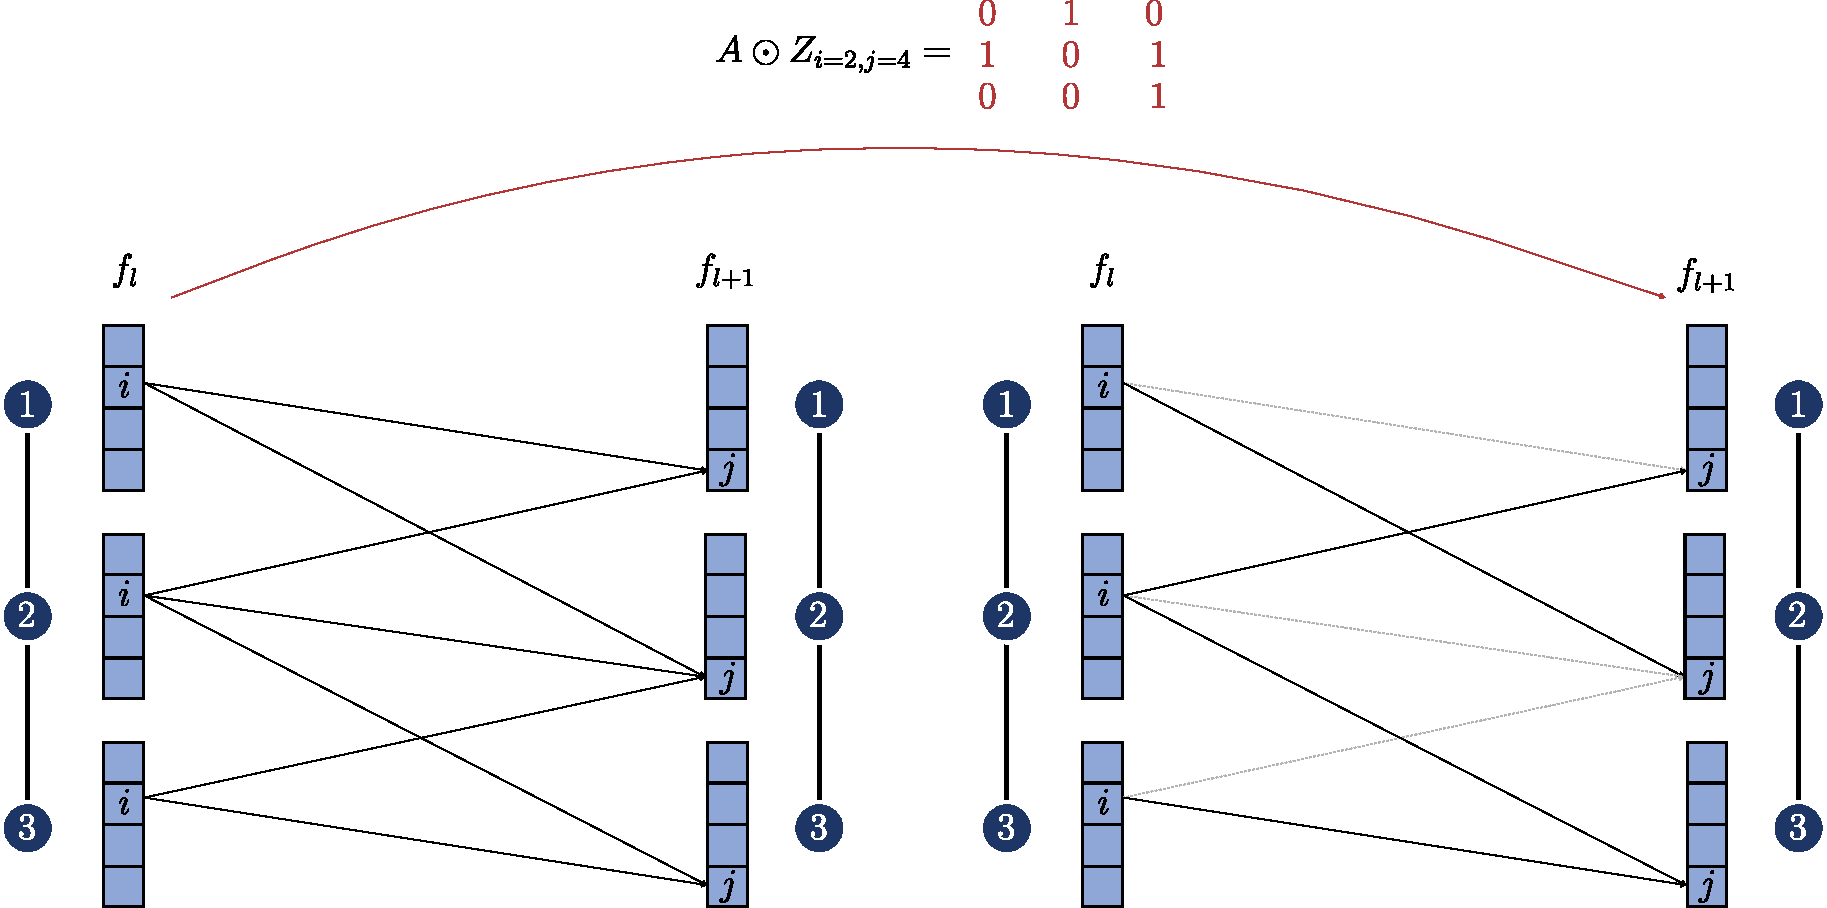
\includegraphics[width= 0.90\linewidth]{gfx/implementation/GDC-eq4.pdf}
    \caption{\Ac{gdc}Note: self connection are assumed}\label{fig:implementaion:GDC-eq4}
\end{figure}


As for the implementation of \ac{gdc}, we decided to implement the less complex version, as shown below, since this implementation reduces the runtime completely and is also the one that was originally implemented for testing the efficacy of \ac{gdc}

\begin{align}
    H^{(l+1)} = \sigma(\sum_{i= 1}^{f_{l}}\mathfrak{N}(A \odot Z_{i}^{(l)})H^{(l)}[:,i] W^{(l)}[i,:]) \label{eq:relaxed}
\end{align}



Here, we compute the new feature matrix in one go instead of doing $f_{l}$ iterations for all $f_{l}$ columns.
\begin{figure}[ht]
    \centering
    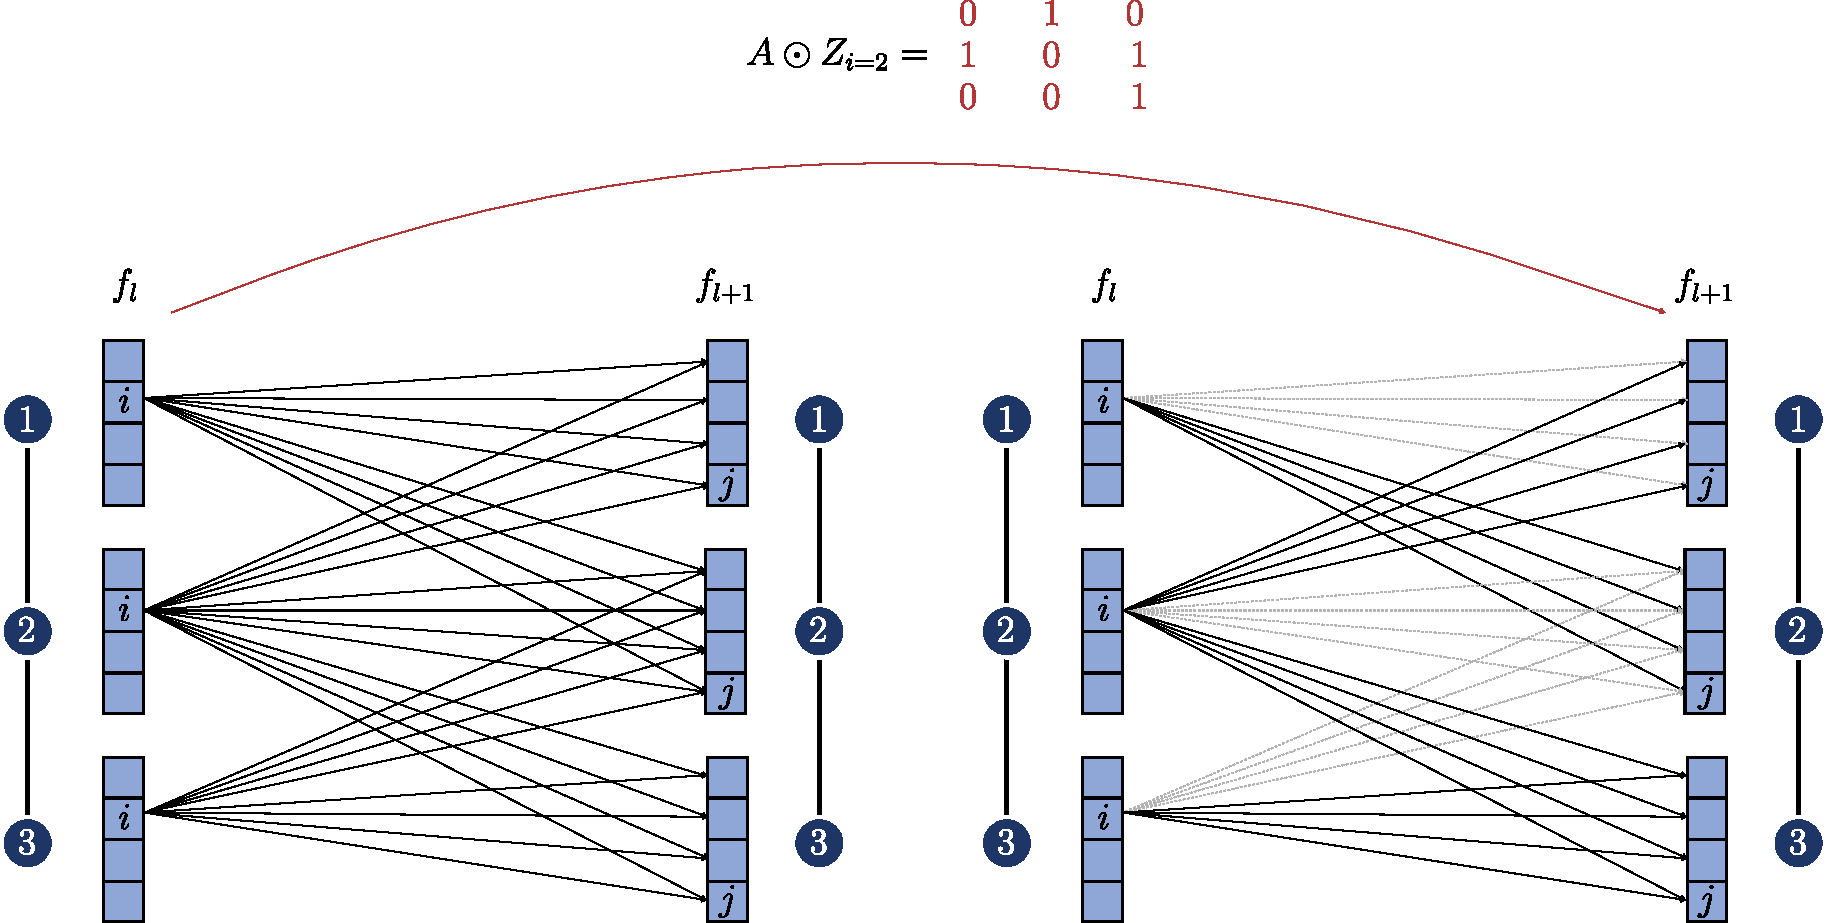
\includegraphics[width= 0.90\linewidth]{gfx/implementation/GDC-eq5.pdf}
    \caption{Originally proposed \ac{gdc}Note: self connection are assumed}\label{fig:implementaion:GDC-eq5}
\end{figure}

\section{Choice of Libraries and Frameworks}
\label{sec:implement:frameworks}
Below, we briefly overview used datasets and frameworks and motivate the choice.
% TODO: Tensorflow
% TODO: NetworkX

% \subsection{Datasets}
% \label{sec:implement:frameworks: datasets}
% Datasets - OGB 
Even though machine learning on graph-structured data is carried out in many areas and has many interesting use cases ranging from social networks to molecular graphs, manifolds, and source code~\cite{Hu2020},
there is no unified framework for working with graph-structured data. Furthermore, commonly used datasets and evaluation procedures suffer from multiple issues that negatively affect the quality of predictions and the reliability of evaluations of models.
Machine learning algorithms rely heavily on data. For a \ac{gnn} to be able to make accurate predictions, there is a need for a sufficient amount of properly prepared training data. Standardized splitting and evaluation methods are needed to compare different models against each other.

% Problems overview 
Today, most of the frequently used graph datasets are extremely small compared to graphs found in real applications. The same datasets, such as Cora, CiteSeer, and PubMed, are used repeatedly to train various models, leading to poor scalability in most cases. Small datasets also make it hard to rigorously evaluate data-hungry models, such as \acfp{gnn}. The performance of a \ac{gnn} on these datasets is often unstable and nearly statistically identical to each other, due to the small number of samples the models are trained and evaluated on~\cite{Kipf2017,Xu2019, Hu2020}.

% OGB benefits  
\textbf{\Ac{ogb}} offers a wide range of different-sized graph datasets from different domains for a variety of varying classification tasks and provides a unified pipeline for working with the datasets in \ac{ml} tasks.
The unified experimental protocol with standardized dataset splits, evaluation metrics, and cross-validation protocols makes it easy to compare performance reported across various studies~\cite{Hu2020}.

% Overview of standardized pipeline 
Working with \ac{ogb} consists of following steps:

\begin{enumerate}
    \item \Ac{ogb} provides realistic, different-scaled graph benchmark datasets that cover different prediction tasks from diverse applications.
    \item Dataset processing and splitting is fully automated. \Ac{ogb} data loaders automatically download and process graphs and further split the datasets in a standardized manner. This is compatible with multiple libraries and provides a library-agnostic option.
    \item This step includes developing an \ac{ml} model to train on the \ac{ogb} datasets.
    \item  \Ac{ogb} evaluates the model in a dataset-dependent manner and outputs the model performance appropriate for the task at hand.
    \item \Ac{ogb} provides public leaderboards to keep track of recent advances.
\end{enumerate}

\begin{figure}[H]
    \centering
    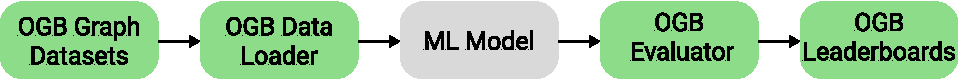
\includegraphics[width= 0.90\linewidth]{gfx/implementation/OGB_pipeline}
    \caption{\textbf{Overview of the standardized OGB pipeline} adapted from \cite{Hu2020}}\label{fig:implement:pipeline}
\end{figure}


%  3.3 Choice of Libraries and Frameworks (mention TensorFlow and NetworkX)
For machine learning tasks, TensorFlow, a powerful and versatile open-source machine learning framework, was a fundamental tool for developing and training intricate machine learning models.
TensorFlow's extensive set of libraries and tools simplifies the process of building, training, and deploying machine learning models, making it a preferred choice.
The framework's adaptability to various tasks, ranging from image recognition to natural language processing, underscores its universal applicability, positioning it at the forefront of modern machine learning research.
In addition to TensorFlow, this study leveraged NetworkX, a Python package designed to create, manipulate, and analyze complex networks. NetworkX was used as a tool for graph representation.
 % INCLUDE:
% !TEX root = ../main.tex
%
\chapter{Evaluation}
\label{sec:eval}

% Is it necessary to quote all the studies here ?? YES
In this section, we delve into the critical evaluation of the machine learning experiments conducted as part of this research.
The main postulated question of this study was to determine whether \ac{gdc} is effective in solving the problem of overfitting and over-smoothing for graph-level prediction tasks, as there is already a wide range of conducted studies, which answer the question of various regularization techniques for node level prediction tasks. Other regularization techniques have also been evaluated for this type of task.
The investigation encompassed classification and regression tasks, with a comprehensive analysis of two types of neural networks, \ac{gcn} and \ac{gin}.
The datasets of choice were all molecular datasets.
In the evaluation, we will mainly focus on two manipulated parameters: the number of layers and the dropout rate, since the number of layers is important in concluding overfitting, especially the issue where additional layers do not make the network perform better. The dropout rate since this parameter indicates the efficacy of various types of dropouts and if higher rates have an impact at all.


\section{Datasets and Metrics Overview}
\label{sec:eval:overvies}

Before proceeding to the experimental findings, we present a quick overview of the used datasets and metrics to ensure a better understanding of the subject matter. We have used five datasets, all from the molecular realm. Molhiv and molpcba are small and medium-size classification datasets, respectively.
The other three, OGB-molesol, -mollipo and -molfreesolv are regression datasets. They contain 1128, 4200, and 642
molecular structure graphs, respectively. The regression task is to predict the solubility
of a molecule in different substances.
To evaluate the performance of molhiv, we used ROC-AUC, for molpcba AP was used and we used MAE for all the regression datasets.

\section{Experimental Setup}
\label{sec:eval:setup}
% Add general training methodology 
% Problem definition 
This section outlines the experimental setup for training the \ac{gcn} and the \ac{gin} network architectures.
We did not have to deal with data preprocessing steps and data preparation techniques because we use the \ac{ogb} datasets~\cite{Hu2020}.

% General training methodology 
The training of the \ac{gnn} models followed a systematic methodology to ensure the robustness and reliability of the results. The following key parameters were considered:
The training process spanned  $N_{epochs}= 200$ to ensure the model can learn the underlying patterns within the data.
Training with each configuration was repeated three times to account for variability in the training process.
Early stopping was used to prevent overfitting and enhance the generalization ability of the models. The training process monitored the validation loss, and the training was halted if the validation loss did not improve for a consecutive number of epochs.
The `patience' parameter was set to 50, indicating that the training process was terminated early if the validation loss did not decrease over 50 consecutive epochs.
The selection of the best hyperparameter configuration was based on the validation loss.
The configuration yielding the lowest validation loss was chosen as the optimal setting among the evaluated hyperparameter combinations.
The Adam optimizer was employed during the training process.

\subsection{Parameter Grid}
In this study, a comprehensive exploration of the model's hyperparameters was conducted to optimize the performance of the graph neural network.
The hyperparameter search space was defined through a parameter grid encompassing various configurations.
It was designed to contain many possibilities, enabling a systematic investigation of the model's behavior under different settings.

This parameter grid contained several layers ranging from 1 to 6, representing the depth of the neural network architecture.
The learning rate alternated between the three different values $0.0001$, $0.001$, and $0.01$ for the optimization of the model.
We chose the Adam optimizer exclusively for its robust performance in optimizing complex neural networks.
As mentioned previously, we looked at four regularization techniques described in \cref{sec:related:pred:regularization}, \ac{do}, \ac{ns}, \ac{de}, \ac{gdc}, and also looked at the performance when no regularization was applied.
The drop probability for each of the performed regularizations was either set to $0.3$, $0.5$, or $0.7$.
We also considered three activation functions: `relu', `sigmoid', and `tanh'.
The number of units in the hidden layer units, determining the neural network's capacity, was alternated between $32$ and $64$.
All this was done for two different network architectures, \ac{gcn} and \ac{gin}.
All possible combinations of these parameters were generated to comprehensively explore the hyperparameter space, resulting in a list denoted as \texttt{param_combos}.
Each configuration within \texttt{param_combos} represented a unique set of hyperparameters for the graph neural network. By exhaustively evaluating these combinations, this study aimed to identify the most suitable hyperparameter configuration, providing valuable insights into the optimal setup for graph-based machine learning tasks.

\subsection{Finding the Best Set of Hyperparameters}
\label{sec:implement:setup: gridsearch}
For hyperparameter optimization, we use grid search \ac{gs}~\cite{Lorenzo2017,Yang2020,Zoeller2021}.\Ac{gs} is a model-free method of automated hyperparameter selection, which systematically explores the configuration space performing an exhaustive search.
Grid search has tow major drawbacks:
\begin{enumerate}
    \item Poor scalability for large configuration spaces due to its exponential complexity in the number of hyperparameters and corresponding values. Assuming that there are k parameters, and each of them has n distinct values, its computational complexity is $O(n^{k})$.
    \item Lack of consideration of the hierarchical hyperparameter structure leads to many redundant configurations.
\end{enumerate}
Despite its two major drawbacks, \ac{gs} is well-suitable for small search spaces and can easily be implemented and parallelized.

\section{Experimental Results}
\label{sec:eval:results}

\begin{table*}[ht]
    \caption{
        Experimental results for graph-level prediction tasks. With ROC-AUC metric for OGB-molhiv, AP for -molpcba and MSE for the three remaining regression datasets.
    }\label{tbl:eval:results}
    \centering
    {\small%\scriptsize%
        \csvreader[
            column count=12,
            tabular={clrrrrr},
            separator=semicolon,
            table head={%
                    & \multicolumn{1}{l}{} &%
                    \multicolumn{1}{c}{\textbf{OGB-molhiv}} &%
                    \multicolumn{1}{c}{\textbf{-molpcba}} &%
                    \multicolumn{1}{c}{\textbf{-molesol}} &%
                    \multicolumn{1}{c}{\textbf{-molfreesolv}} &%
                    \multicolumn{1}{c}{\textbf{-mollipo}}%
                    \\\toprule%
                },
            before reading={\setlength{\tabcolsep}{4pt}},
            table foot=\bottomrule,
            late after line=\ifthenelse{\equal{\id}{5}}{\\\midrule}{\\},
            head to column names
        ]{data/results.csv}{}{%
            \ifthenelse{\equal{\id}{0}}{\multirow{5}{*}[0em]{\rotatebox[origin=c]{90}{\textsc{GCN}}}}{}%
            \ifthenelse{\equal{\id}{5}}{\multirow{5}{*}[0em]{\rotatebox[origin=c]{90}{\textsc{GIN}}}}{}&%
            \textbf{\regularization} &%
            {\evalres{0}{\molhivAvg}{\molhivStd}} &%
            {\evalres{0}{\molpcbaAvg}{\molpcbaStd}} &%
            {\evalres{0}{\molesolAvg}{\molesolStd}} &%
            {\evalres{0}{\molfreesolvAvg}{\molfreesolvStd}} &%
            {\evalres{0}{\mollipoAvg}{\mollipoStd}}%
        }}
\end{table*}

% % Description of results - Basic overview 
% Our experiments produced the following results:
% Basic first view insights: 
As seen in \cref{tbl:eval:results}, the best results are achieved using no regularization techniques for graph-level prediction tasks on both types of networks \ac{gcn} and \ac{gin}.
This holds for both datasets -- classification and regression -- indicating that any regularization type is unsuitable for both graph-level prediction tasks independently of the network of choice.
For both classification datasets, the variance is very small; the network performance is stable. Out of the three regression datasets, only the mollipo dataset has low variance in performance for both types of \acp{gnn}, and we have rather a high variance on the remaining datasets.
The high variance of molesol and mollipo is an interesting trend, which would be nice to investigate further.
% Patterns Among the datasets 
Despite achieving the best result when using no regularization, we can point out a clear second-place winner among the different regularization methods on both networks and across all datasets.
\Ac{de} performs the second best in all cases, with the second place being \ac{gdc} for classification tasks and \ac{ns} for regression tasks, apart from one exception on the mollipo dataset where the second best performing regularization is \ac{gdc}.
However, as all the results are very close in range, we cannot point out any notable advantages of using \ac{gdc} above other regularization methods, as their performance varies depending on the task and dataset.
% Other noteworthy things  
Despite the \ac{gin} network being more powerful than \ac{gcn} and as powerful as the 1-dim.\ \ac{wl} test, the performance on both networks is very similar, with only a significant difference in performance on the molhiv dataset.

\newcommand*{\addstd}[4]{
    \addplot[name path=#3upper, draw=none] table[x=#2, y expr=\thisrow{#3Avg}+\thisrow{#3Std}, col sep=semicolon] {#1};
    \addplot[name path=#3lower, draw=none] table[x=#2, y expr=\thisrow{#3Avg}-\thisrow{#3Std}, col sep=semicolon] {#1};
    \addplot[fill=#4, fill opacity=0.1] fill between[of=#3upper and #3lower];
}
\newcommand*{\layerplot}[6]{\begin{tikzpicture}
        \begin{axis}[
                width=0.8\linewidth,
                height=6cm,
                xlabel={#3},
                ylabel={#4},
                xtick={#5}, % Set x-axis tick distance
                ytick distance={#6}, % Set y-axis tick distance
                legend pos=outer north east,
                legend style={nodes={scale=0.6, transform shape}},
                grid=major,
            ]

            % Plot the data from the CSV file
            \addplot[color= p_red] table [x=#2, y=noneAvg, col sep=semicolon] {#1};
            \addlegendentry{No Regularization}

            \addplot[color= p_green] table [x=#2, y=dropoutAvg, col sep=semicolon] {#1};
            \addlegendentry{Dropout}

            \addplot[color= p_blue] table [x=#2, y=nodesamplingAvg, col sep=semicolon] {#1};
            \addlegendentry{Node Sampling}

            \addplot[color= p_yellow] table [x=#2, y=dropedgeAvg, col sep=semicolon] {#1};
            \addlegendentry{DropEdge}

            \addplot[color= p_violet] table [x=#2, y=gdcAvg, col sep=semicolon] {#1};
            \addlegendentry{GDC}

            \addstd{#1}{#2}{none}{p_red}
            \addstd{#1}{#2}{dropout}{p_green}
            \addstd{#1}{#2}{nodesampling}{p_blue}
            \addstd{#1}{#2}{dropedge}{p_yellow}
            \addstd{#1}{#2}{gdc}{p_violet}
        \end{axis}
    \end{tikzpicture}}


\section{Detailed Investigation of Change in Number of Layers and Probability}
Since we could not detect any benefits of using regularization for graph-level prediction tasks, indicating that the potential reduction of over-smoothing shown by \citep{Hasanzadeh2020} is not relevant for graph-level prediction tasks.
Therefore, we focus on over-fitting and investigate how the model performance changes when we increase the number of layers.
Also, we want to make sure that our findings are consistent with and can be attributed to the use of regularization, which is why we take a look at the change of performance with regards to drop probability.

\subsection{Effect of the Number of Layers}
This analysis aims to gain insights into the phenomenon of over-smoothing. To achieve this, we investigate the variations in performance corresponding to changes in the number of layers within the network architecture.
Upon analyzing five distinct datasets, discernible patterns in performance relative to the number of network layers become evident. Except for the molhiv and molfreesolv datasets, a weak positive correlation between increased layers and improved performance is observable. This trend is consistent across both \ac{gcn} and \ac{gin} models. Typically, optimal performance is achieved at the 5th or 6th layer. However, it is noteworthy that the overall differences in performance are marginal.

This observed trend persists across various regularization techniques, including scenarios without regularization.
Interestingly, there is insufficient evidence for the hypothesis that regularization effectively mitigates over-smoothing for graph-level classification tasks on \acp{gcn}, specifically concerning these datasets.
Additionally, substantial fluctuations are observed in the molhiv dataset, so no clear trends could be found.

In regression datasets, the molfreesolv dataset presents a unique case where optimal performance is attained with a single layer, contrary to the general trend where 5-6 layers yield high performance. Importantly, consistent trends emerge across all regularization techniques and without regularization, suggesting that regularization does not induce unexpected network behavior.

Regarding variance, apart from substantial variance and high fluctuations observed in the molhiv dataset, across both networks and all types of regularization, including scenarios without any regularization, we can observe somewhat clear trends most of the time.
Overall, higher variance is evident in instances without regularization, whereas regularization techniques tend to stabilize performance, resulting in lower variance. This finding underscores the stabilizing influence of regularization techniques on model performance in graph-level classification tasks.

% Classification Datasets Num Layers
% \begin{figure}
%     \centering
%     \layerplot{data/num_layers_plot_molhiv_gcn.csv}{numLayers}{Number of Layers}{ROC-AUC}{1,2,3,4,5,6}{0.1}
%     \caption{molhiv (GCN Model)}
% %     \label{fig:layers-gcn-molhiv}
% \end{figure}

\begin{figure}
    \centering
    \layerplot{data/num_layers_plot_molpcba_gcn.csv}{numLayers}{Number of Layers}{AP}{1,2,3,4,5,6}{0.02}
    \caption{molpcba (GCN Model)}
    \label{fig:layers-prob-gcn-molpcba}
\end{figure}


\begin{figure}
    \centering
    \layerplot{data/num_layers_plot_molesol_gcn.csv}{numLayers}{Number of Layers}{MSE}{1,2,3,4,5,6}{1}
    \caption{molesol (GCN Model)}
    \label{fig:layers-gcn-molesol}
\end{figure}

% \begin{figure}
%     \centering
%     \layerplot{data/num_layers_plot_molfreesolv_gcn.csv}{numLayers}{Number of Layers}{MSE}{1,2,3,4,5,6}{5}
%     \caption{molfreesolv (GCN Model)}
%     \label{fig:layers-gcn-molfreesolv}
% \end{figure}

\begin{figure}
    \centering
    \layerplot{data/num_layers_plot_mollipo_gcn.csv}{numLayers}{Number of Layers}{MSE}{1,2,3,4,5,6}{0.2}
    \caption{mollipo (GCN Model)}
    \label{fig:layers-gcn-mollipo}
\end{figure}

% Regression Datasets Insights Num Layers 
% \begin{figure}
%     \centering
%     \layerplot{data/num_layers_plot_molhiv_gin.csv}{numLayers}{Number of Layers}{ROC-AUC}{1,2,3,4,5,6}{0.1}
%     \caption{molhiv (GIN Model)}
%     \label{fig:layers-gin-molhiv}
% \end{figure}

% \begin{figure}
%     \centering
%     \layerplot{data/num_layers_plot_molpcba_gin.csv}{numLayers}{Number of Layers}{AP}{1,2,3,4,5,6}{0.95}
%     \caption{molpcba (GIN Model)}
%     \label{fig:layers-gin-molpcba}
% \end{figure}

% % Regression Datasets Insights 
% \begin{figure}
%     \centering
%     \layerplot{data/num_layers_plot_molesol_gin.csv}{numLayers}{Number of Layers}{MSE}{1,2,3,4,5,6}{1}
%     \caption{molesol (GIN Model)}
%     \label{fig:layers-gin-molesol}
% \end{figure}

\begin{figure}
    \centering
    \layerplot{data/num_layers_plot_molfreesolv_gin.csv}{numLayers}{Number of Layers}{MSE}{1,2,3,4,5,6}{5}
    \caption{molfreesolv (GIN Model)}
    \label{fig:layers-gin-molfreesolv}
\end{figure}

% \begin{figure}
%     \centering
%     \layerplot{data/num_layers_plot_mollipo_gin.csv}{numLayers}{Number of Layers}{MSE}{1,2,3,4,5,6}{0.2}
%     \caption{mollipo (GIN Model)}
%     \label{fig:layers-gin-mollipo}
% \end{figure}

% Here are the regression datasets 
\subsection{Effect of the Probability of Regularization}

We also take a closer look at how a change in the drop probability affects the performance of the networks.
Regarding this, we have found that the model performs worse on average as we approach higher probabilities, i.e., a lower dropout probability leads to better performance.
This makes sense, as the best performance is achieved using no regularization.
This trend can be observed in the regression datasets on the \ac{gcn} and the \ac{gin}network. This trend also holds for the classification dataset molpcba on both networks. On the molhiv dataset, the dropout probability does not lead to any substantial differences in performance, which is why we do not show it.

% \begin{figure}
%     \centering
%     \layerplot{data/probability_plot_molhiv_gcn.csv}{probability}{Probability}{ROC-AUC}{0.3, 0.5, 0.7}{0.1}
%     \caption{molhiv (GCN Model)}
%     \label{fig:prob-gcn-molfreesolv}
% \end{figure}

\begin{figure}
    \centering
    \layerplot{data/probability_plot_molpcba_gcn.csv}{probability}{Probability}{AP}{0.3, 0.5, 0.7}{0.02}
    \caption{molpcba (GCN Model)}
    \label{fig:prob-gcn-molpcba}
\end{figure}

\begin{figure}
    \centering
    \layerplot{data/probability_plot_molesol_gcn.csv}{probability}{Probability}{MSE}{0.3, 0.5, 0.7}{1}
    \caption{molesol (GCN Model)}
    \label{fig:prob-gcn-molesol}
\end{figure}

% \begin{figure}
%     \centering
%     \layerplot{data/probability_plot_molfreesolv_gcn.csv}{probability}{Probability}{MSE}{0.3, 0.5, 0.7}{2}
%     \caption{molfreesolv (GCN Model)}
%     \label{fig:prob-gcn-molfreesolv}
% \end{figure}

\begin{figure}
    \centering
    \layerplot{data/probability_plot_mollipo_gcn.csv}{probability}{Probability}{MSE}{0.3, 0.5, 0.7}{0.2}
    \caption{mollipo (GCN Model)}
    \label{fig:prob-gcn-mollipo}
\end{figure}

% HERE ARE THE DATASETS FOR PROBABiLITY ON GIN 
% \begin{figure}
%     \centering
%     \layerplot{data/probability_plot_molhiv_gin.csv}{probability}{Probability}{ROC-AUC}{0.3, 0.5, 0.7}{0.1}
%     \caption{molhiv (GIN Model)}
%     \label{fig:prob-gin-molhiv}
% \end{figure}

% \begin{figure}
%     \centering
%     \layerplot{data/probability_plot_molpcba_gin.csv}{probability}{Probability}{AP}{0.3, 0.5, 0.7}{0.02}
%     \caption{molpcba (GIN Model)}
%     \label{fig:prob-gin-molpcba}
% \end{figure}

% \begin{figure}
%     \centering
%     \layerplot{data/probability_plot_molesol_gin.csv}{probability}{Probability}{MSE}{0.3, 0.5, 0.7}{1}
%     \caption{molesol (GIN Model)}
%     \label{fig:prob-gin-molesol}
% \end{figure}

\begin{figure}
    \centering
    \layerplot{data/probability_plot_molfreesolv_gin.csv}{probability}{Probability}{MSE}{0.3, 0.5, 0.7}{2}
    \caption{molfreesolv (GIN Model)}
    \label{fig:prob-gin-molfreesolv}
\end{figure}

% \begin{figure}
%     \centering
%     \layerplot{data/probability_plot_mollipo_gin.csv}{probability}{Probability}{MSE}{0.3, 0.5, 0.7}{0.2}
%     \caption{mollipo (GIN Model)}
%     \label{fig:prob-gin-mollipo}
% \end{figure}


% Patterns of variance in datasets 

Among the datasets, the classification dataset molhiv and the regression dataset molfreesoolv

% Overall Conclusion for the number of layers/ regularization 
As mentioned earlier, the results are very close in range, and together with the limited number of datasets- all from the same molecular realm- we cannot draw any general conclusions. However, we can describe some emerging trends from our findings:
The trends:
Overall, regularization seems to smoothen the line, i.e., to reduce the differences in performance depending on the number of layers. Also, the performance variance is much higher when we use no regularization.




% !TEX root = ../main.tex
%
\chapter{Conclusion}
\label{sec:conclusion}

% Structure
% Review 
% Outlook 

% To be placed 


\section{Review}
\label{sec:conclusion:review}

Our study examined the impact of various regularization techniques, particularly \ac{gdc}, on graph-level prediction tasks across two different network types.
Specifically, we postulated the following three research questions, which we will now answer.

% Here come explicit answers to all the research questions
\paragraph{RQ1: Is regularization, specifically \acs*{gdc}, effective in solving the problem of over-fitting and over-smoothing for graph-level prediction tasks?}
Since both our networks had no problem with over-fitting, even if no regularization was used, we cannot say anything about the effectiveness of regularization in mitigating this problem.
We can only say that the model is not negatively affected by regularization in terms of over-smoothing.

\paragraph{RQ2: Is there a difference in performance between \acs*{gcn} and \acs*{gin} architectures regarding performance with regularization techniques?}

We found no difference in performance between both network architectures \ac{gcn} and \ac{gin}.
Both networks perform best when we use no regularization at all, and on both networks, \ac{de} is the second-best performance most of the time.
This holds for both classification and regression datasets.


\paragraph{RQ3: Are there similarities and differences between different regularization techniques in terms of performance?}
We tried to verify or refute whether any of the four regularization techniques \ac{do}, \ac{ns}, \ac{de}, and \ac{gdc} is more effective.
In terms of performance, the different regularization techniques are very close.
\Ac{de} performs best among the different datasets and \ac{gdc} is second-place, hinting at the close relatedness between those two techniques, as already has been described by \citep{Hasanzadeh2020}.


\section{Future Work}
\label{sec:conclusion:future}

Our investigation observed that regularization might not offer significant advantages for graph-level prediction tasks, opening avenues for further exploration, which leads to intriguing questions that warrant deeper investigation.
While our study focused on two widely employed \ac{gnn}architectures, \ac{gcn} and \ac{gin}, it is crucial to acknowledge the limitations of our experiments, which were conducted on a limited number of datasets.
The generalizability of our findings to other datasets remains an open question, and we encourage researchers to extend our work to explore potential variations in results across diverse datasets.

In our study, we stumbled upon an interesting metric \ac{mad}, which measures the similarity between nodes and allows us to gain deeper insights into how and when over-smoothing occurs.
Regrettably, due to the expansive nature of this research, we could not comprehensively evaluate \ac{mad} within the scope of this study.
We advocate for further research to assess the efficacy of \ac{mad} in graph-level prediction tasks.
Additionally, our exploration hints at alternative regularization techniques that may yield promising results.
\texttt{Noisy Nodes}, a particularly intriguing regularization approach, in which the input graph is corrupted with noise and a noise-correcting node-level loss is added \cref{God22}.

In conclusion, while our study sheds light on the limited efficacy of traditional regularization methods, it also lays the groundwork for future research directions.
We hope that our findings stimulate further inquiry into the nuances of graph-level prediction tasks, focusing on evaluating \ac{mad} and exploring alternative regularization techniques, such as \texttt{Noisy Nodes}, to advance the field and deepen our understanding of graph-based machine learning models.
% Another proposed regularization technique:
% https://arxiv.org/pdf/2106.07971.pdf     % INCLUDE: conclusion
% --------------------------
% Back matter
% --------------------------
\appendix\cleardoublepage\
%\input{content/chapter-appendix}
\cleardoublepage\
%
{%
\setstretch{1.1}
\renewcommand{\bibfont}{\normalfont\small}
\setlength{\biblabelsep}{0pt}
\setlength{\bibitemsep}{0.5\baselineskip plus 0.5\baselineskip} % chktex 1
\setcounter{biburllcpenalty}{9000}
\setcounter{biburlucpenalty}{9999}
\printbibliography[nottype=online]
\printbibliography[heading=subbibliography,title={Websites},type=online]
}
\cleardoublepage

\listoffigures
\cleardoublepage

\listoftables
\cleardoublepage

\input{content/colophon}
\cleardoublepage

% !TEX root = ../main.tex
%
%************************************************
% Declaration
%************************************************
\begin{otherlanguage}{ngerman}
	\pdfbookmark[0]{Declaration}{Declaration}
	\chapter*{Declaration}
	\label{sec:declaration}
	\thispagestyle{empty}

	Ich, Olga Yakobson (Matrikel-Nr. 11591478), versichere, dass ich die Masterarbeit mit
	dem Thema \emph{\thesisTitle} selbstständig verfasst und keine
	anderen als die angegebenen Quellen und Hilfsmittel benutzt habe. Die Stellen der
	Arbeit, die ich anderen Werken dem Wortlaut oder dem Sinn nach entnommen habe,
	wurden in jedem Fall unter Angabe der Quellen der Entlehnung kenntlich gemacht.
	Das Gleiche gilt auch für Tabellen, Skizzen, Zeichnungen, bildliche Darstellungen
	usw. Die Bachelorarbeit habe ich nicht, auch nicht auszugsweise, für eine andere
	abgeschlossene Prüfung angefertigt. Auf § 63 Abs.\ 5 HZG wird hingewiesen.
	\bigskip

	\noindent\textit{\thesisUniversityCity, \thesisDate}

	\smallskip

	\begin{flushright}
		\begin{minipage}{5cm}
			\rule{\textwidth}{1pt}
			\centering\thesisName
		\end{minipage}
	\end{flushright}
\end{otherlanguage}
%*****************************************
%*****************************************

\clearpage
\newpage
\mbox{}

% **************************************************
% End of Document CONTENT
% **************************************************
\end{document}
